\documentclass{beamer}\usepackage[]{graphicx}\usepackage[]{color}
%% maxwidth is the original width if it is less than linewidth
%% otherwise use linewidth (to make sure the graphics do not exceed the margin)
\makeatletter
\def\maxwidth{ %
  \ifdim\Gin@nat@width>\linewidth
    \linewidth
  \else
    \Gin@nat@width
  \fi
}
\makeatother

\definecolor{fgcolor}{rgb}{0.345, 0.345, 0.345}
\newcommand{\hlnum}[1]{\textcolor[rgb]{0.686,0.059,0.569}{#1}}%
\newcommand{\hlstr}[1]{\textcolor[rgb]{0.192,0.494,0.8}{#1}}%
\newcommand{\hlcom}[1]{\textcolor[rgb]{0.678,0.584,0.686}{\textit{#1}}}%
\newcommand{\hlopt}[1]{\textcolor[rgb]{0,0,0}{#1}}%
\newcommand{\hlstd}[1]{\textcolor[rgb]{0.345,0.345,0.345}{#1}}%
\newcommand{\hlkwa}[1]{\textcolor[rgb]{0.161,0.373,0.58}{\textbf{#1}}}%
\newcommand{\hlkwb}[1]{\textcolor[rgb]{0.69,0.353,0.396}{#1}}%
\newcommand{\hlkwc}[1]{\textcolor[rgb]{0.333,0.667,0.333}{#1}}%
\newcommand{\hlkwd}[1]{\textcolor[rgb]{0.737,0.353,0.396}{\textbf{#1}}}%

\usepackage{framed}
\makeatletter
\newenvironment{kframe}{%
 \def\at@end@of@kframe{}%
 \ifinner\ifhmode%
  \def\at@end@of@kframe{\end{minipage}}%
  \begin{minipage}{\columnwidth}%
 \fi\fi%
 \def\FrameCommand##1{\hskip\@totalleftmargin \hskip-\fboxsep
 \colorbox{shadecolor}{##1}\hskip-\fboxsep
     % There is no \\@totalrightmargin, so:
     \hskip-\linewidth \hskip-\@totalleftmargin \hskip\columnwidth}%
 \MakeFramed {\advance\hsize-\width
   \@totalleftmargin\z@ \linewidth\hsize
   \@setminipage}}%
 {\par\unskip\endMakeFramed%
 \at@end@of@kframe}
\makeatother

\definecolor{shadecolor}{rgb}{.97, .97, .97}
\definecolor{messagecolor}{rgb}{0, 0, 0}
\definecolor{warningcolor}{rgb}{1, 0, 1}
\definecolor{errorcolor}{rgb}{1, 0, 0}
\newenvironment{knitrout}{}{} % an empty environment to be redefined in TeX

\usepackage{alltt}

\usetheme{CVille}
\usecolortheme{cavs}

\usepackage{multicol}
\usepackage{ulem}

\title{Efficiently Exploring Multilevel Data with Recursive Partitioning}

\author[Daniel P. Martin]{
Daniel P. Martin\\
University of Virginia\\
}

\institute[\textbf{\insertframenumber \hspace{0.1 cm}of \inserttotalframenumber}] 

\date{May 26, 2015}

\pgfdeclareimage[height = 0.5 cm]{university-logo}{UVA}
\logo{\pgfuseimage{university-logo}}
\IfFileExists{upquote.sty}{\usepackage{upquote}}{}
\begin{document}

% rm(list = ls())
% setwd("~/Documents/college stuffs/grad school/Research/Dissertation/Proposal/Presentation/")
% set.seed(42)



%%%%%%%%%%%%%%%%%%%%%%%%%%%%%%%%%%%%%%%%%%%%%%%%%

\begin{frame}

\titlepage

\end{frame}

%%%%%%%%%%%%%%%%%%%%%%%%%%%%%%%%%%%%%%%%%%%%%%%%%

\begin{frame}
\frametitle{Outline}

\begin{itemize}
\item Exploratory data analysis discussion
\item Intro to recursive partitioning
\item Multilevel extensions
\item Multilevel issues (and ``best practices'')
\end{itemize}

\end{frame}

%%%%%%%%%%%%%%%%%%%%%%%%%%%%%%%%%%%%%%%%%%%%%%%%%

\section{EDA Discussion}
\begin{frame}

\begin{quote}
    The term ``exploratory'' is considered by many as less than an approach to data analysis and more a confession of guilt.
\end{quote}

\hspace{6ex} -Jack McArdle, 2014

\pause

\vspace{5ex}

Why is exploratory research seen in this way? How do you use exploratory research (if at all)?

\end{frame}

%%%%%%%%%%%%%%%%%%%%%%%%%%%%%%%%%%%%%%%%%%%%%%%%%

\begin{frame}
\frametitle{What Typically Comes After Confirmatory Tests?}

\begin{center}
Data-driven exploration with NHST
\end{center}

\vspace{-15px}

\begin{center}

\includegraphics[height = 2in]{figure/exploration.jpg}
\end{center}

\end{frame}

%%%%%%%%%%%%%%%%%%%%%%%%%%%%%%%%%%%%%%%%%%%%%%%%%

\begin{frame}
\frametitle{If Not NHST, What Else Is There?}
\framesubtitle{Breiman (2001)}

\begin{center}
Data modeling:
\end{center}

\begin{center}
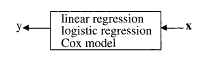
\includegraphics[width = 2in]{figure/data_model.png}
\end{center}

\begin{center}
vs.
\end{center}

\begin{center}
Algorithmic modeling:
\end{center}

\begin{center}
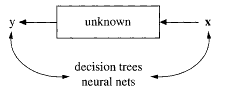
\includegraphics[width = 2in]{figure/algo_model.png}
\end{center}

\end{frame}

%%%%%%%%%%%%%%%%%%%%%%%%%%%%%%%%%%%%%%%%%%%%%%%%%

\section{Recursive Partitioning}
\begin{frame}
\frametitle{An Introduction to Decision Trees}

\begin{knitrout}
\definecolor{shadecolor}{rgb}{0.969, 0.969, 0.969}\color{fgcolor}
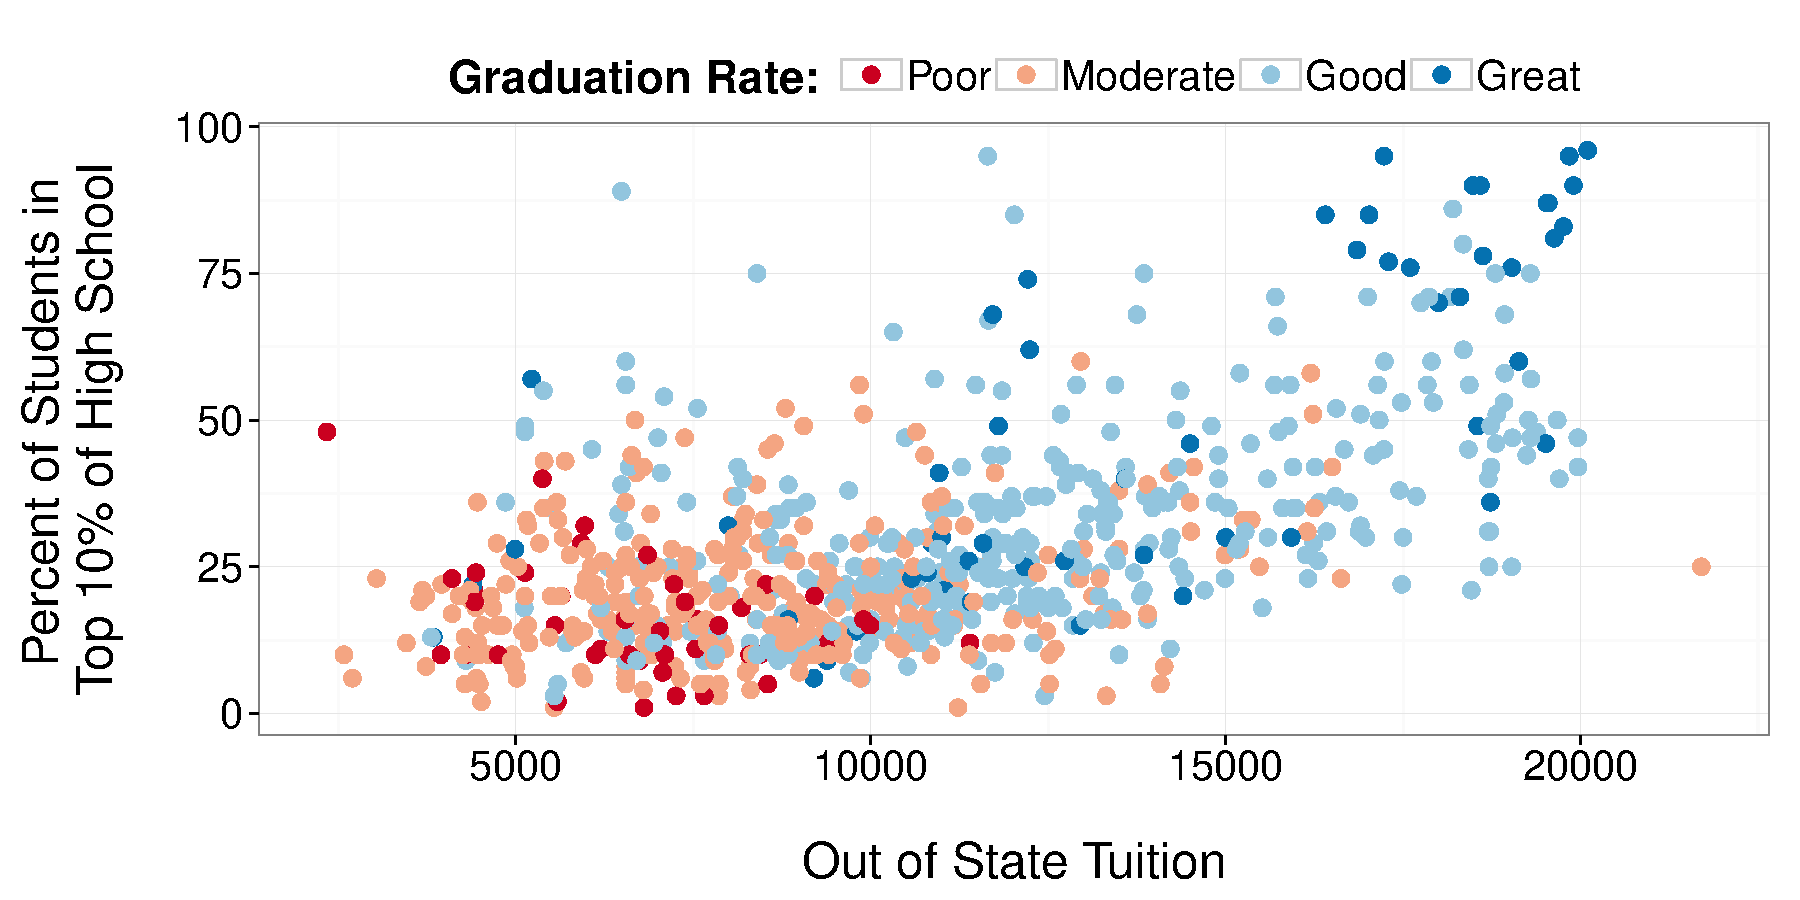
\includegraphics[width=\maxwidth]{figure/grad_rate-1} 

\end{knitrout}

\pause

\centering
$RSS_{total} \stackrel{?}{<} RSS_{part1} + RSS_{part2}$

\end{frame}

%%%%%%%%%%%%%%%%%%%%%%%%%%%%%%%%%%%%%%%%%%%%%%%%%

\begin{frame}
\frametitle{An Introduction to Decision Trees}

\begin{knitrout}
\definecolor{shadecolor}{rgb}{0.969, 0.969, 0.969}\color{fgcolor}
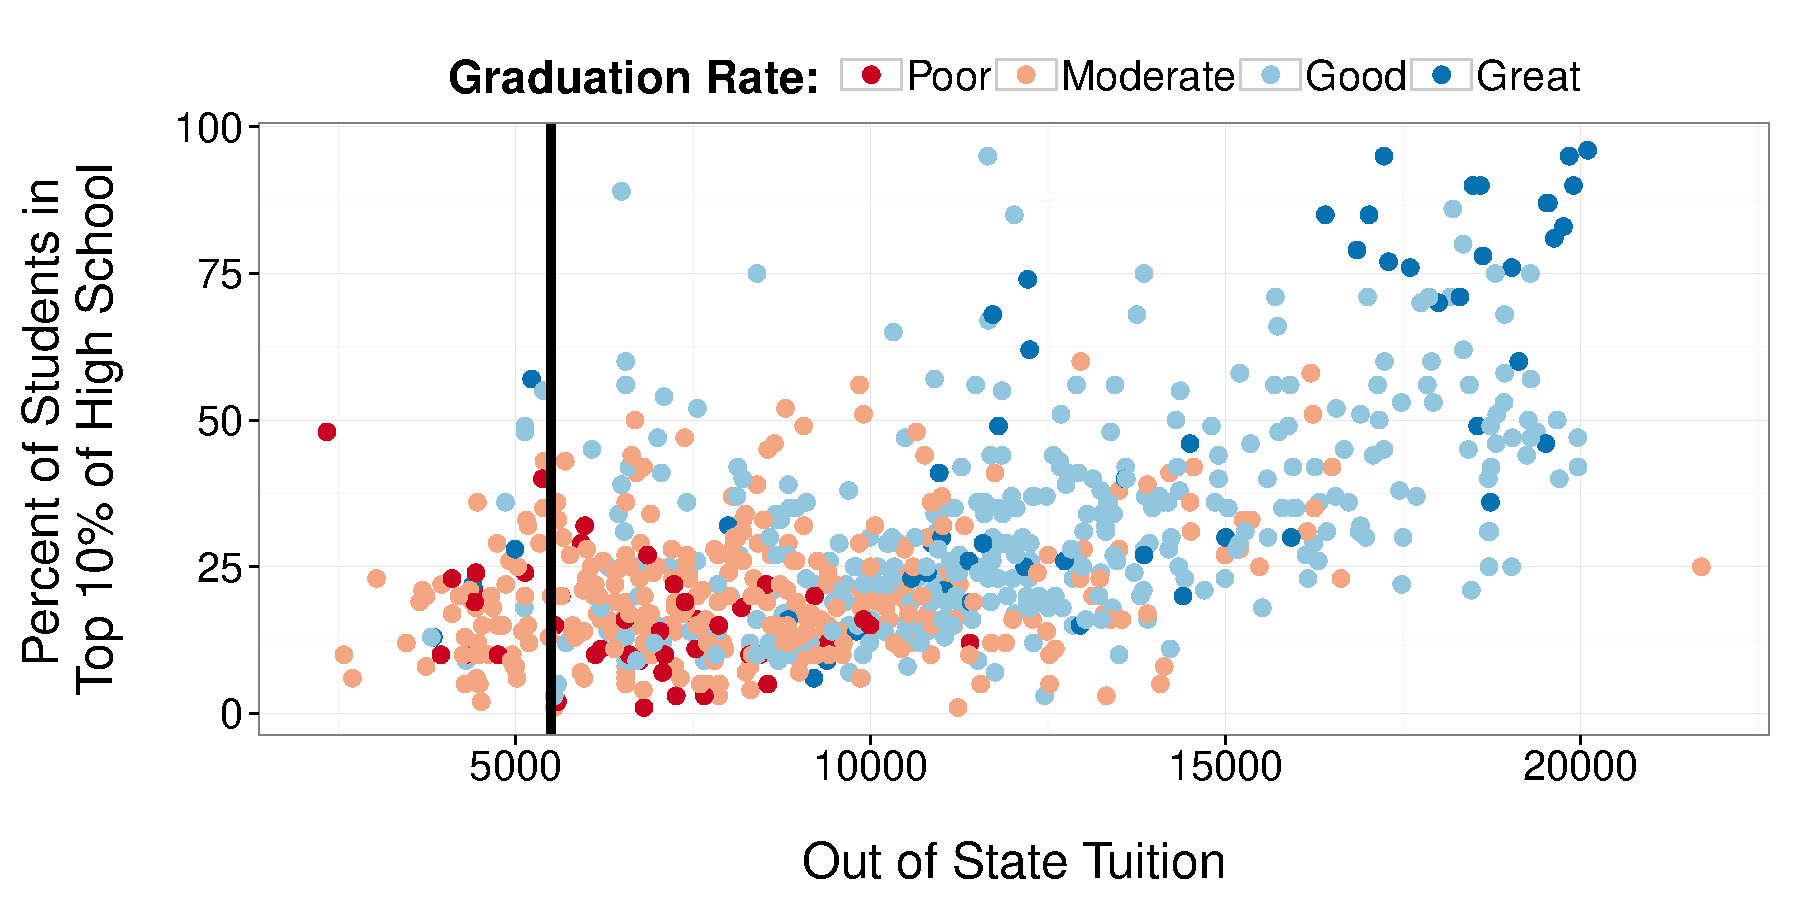
\includegraphics[width=\maxwidth]{figure/grad_rate_try_split-1} 

\end{knitrout}

\vspace{2ex}

\centering
$229 \stackrel{?}{<} 19 + 195 = 215$

\end{frame}

%%%%%%%%%%%%%%%%%%%%%%%%%%%%%%%%%%%%%%%%%%%%%%%%%

\begin{frame}
\frametitle{An Introduction to Decision Trees}

\begin{knitrout}
\definecolor{shadecolor}{rgb}{0.969, 0.969, 0.969}\color{fgcolor}
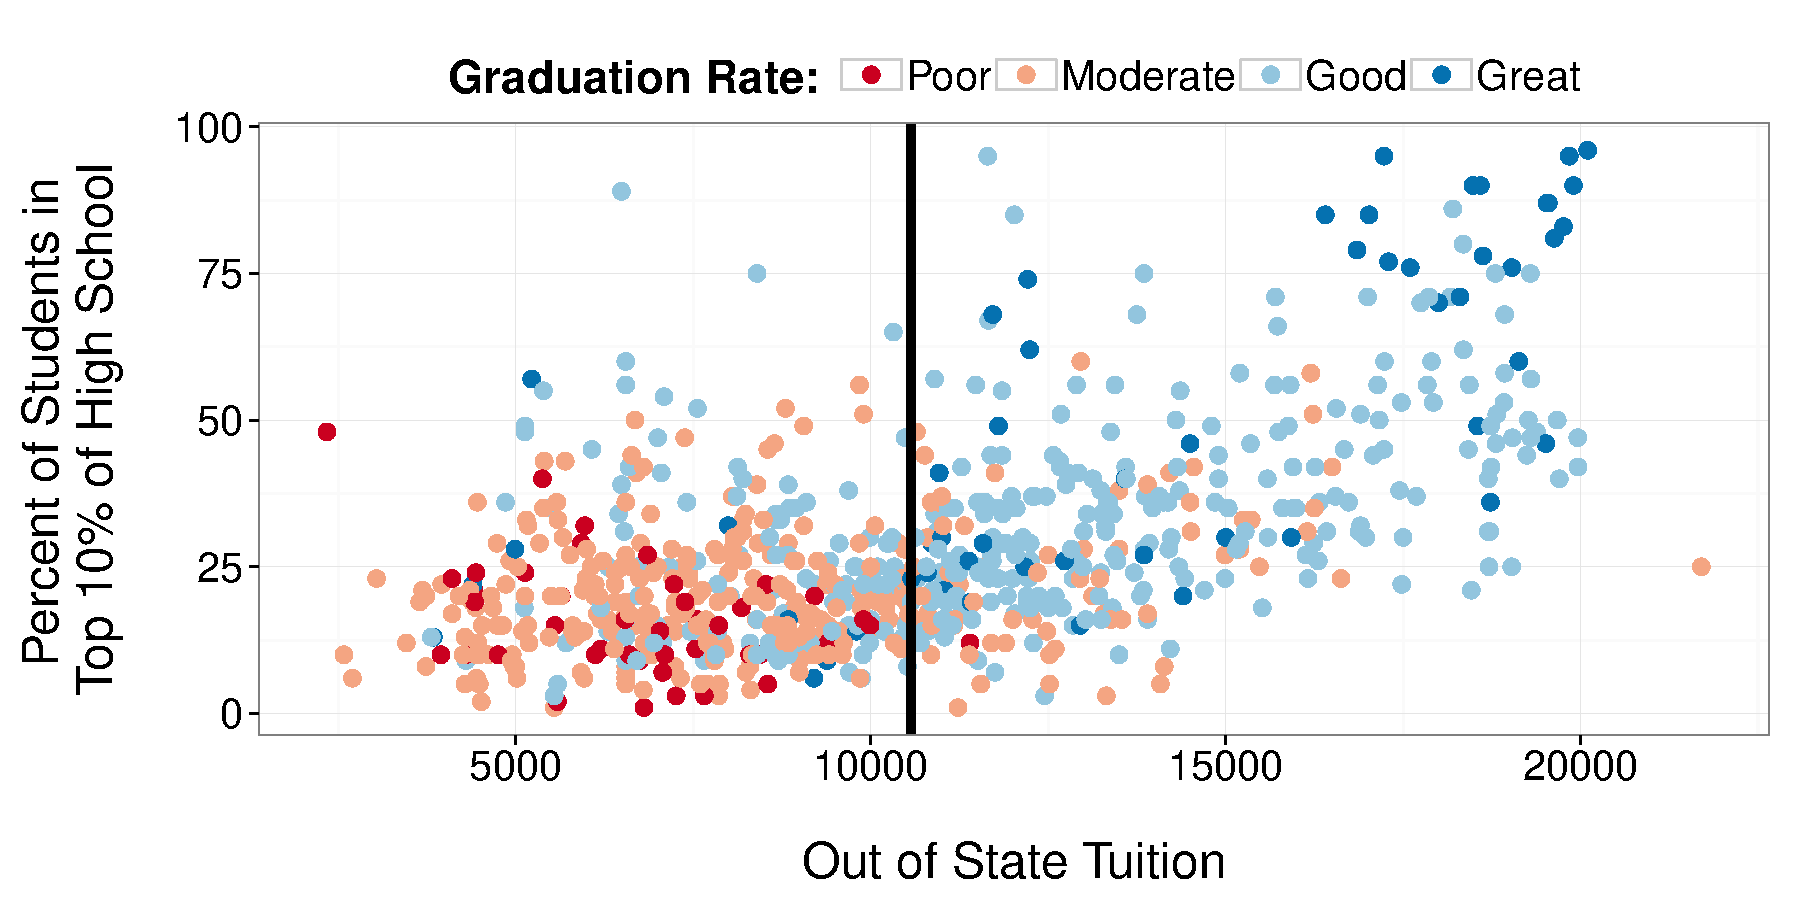
\includegraphics[width=\maxwidth]{figure/grad_rate_best_split-1} 

\end{knitrout}

\vspace{2ex}

\centering
$229 \stackrel{?}{<} 104 + 63 = 168$

\end{frame}

%%%%%%%%%%%%%%%%%%%%%%%%%%%%%%%%%%%%%%%%%%%%%%%%%

\begin{frame}
\frametitle{An Introduction to Decision Trees}

\begin{multicols}{2}

\begin{center}

\begin{knitrout}
\definecolor{shadecolor}{rgb}{0.969, 0.969, 0.969}\color{fgcolor}
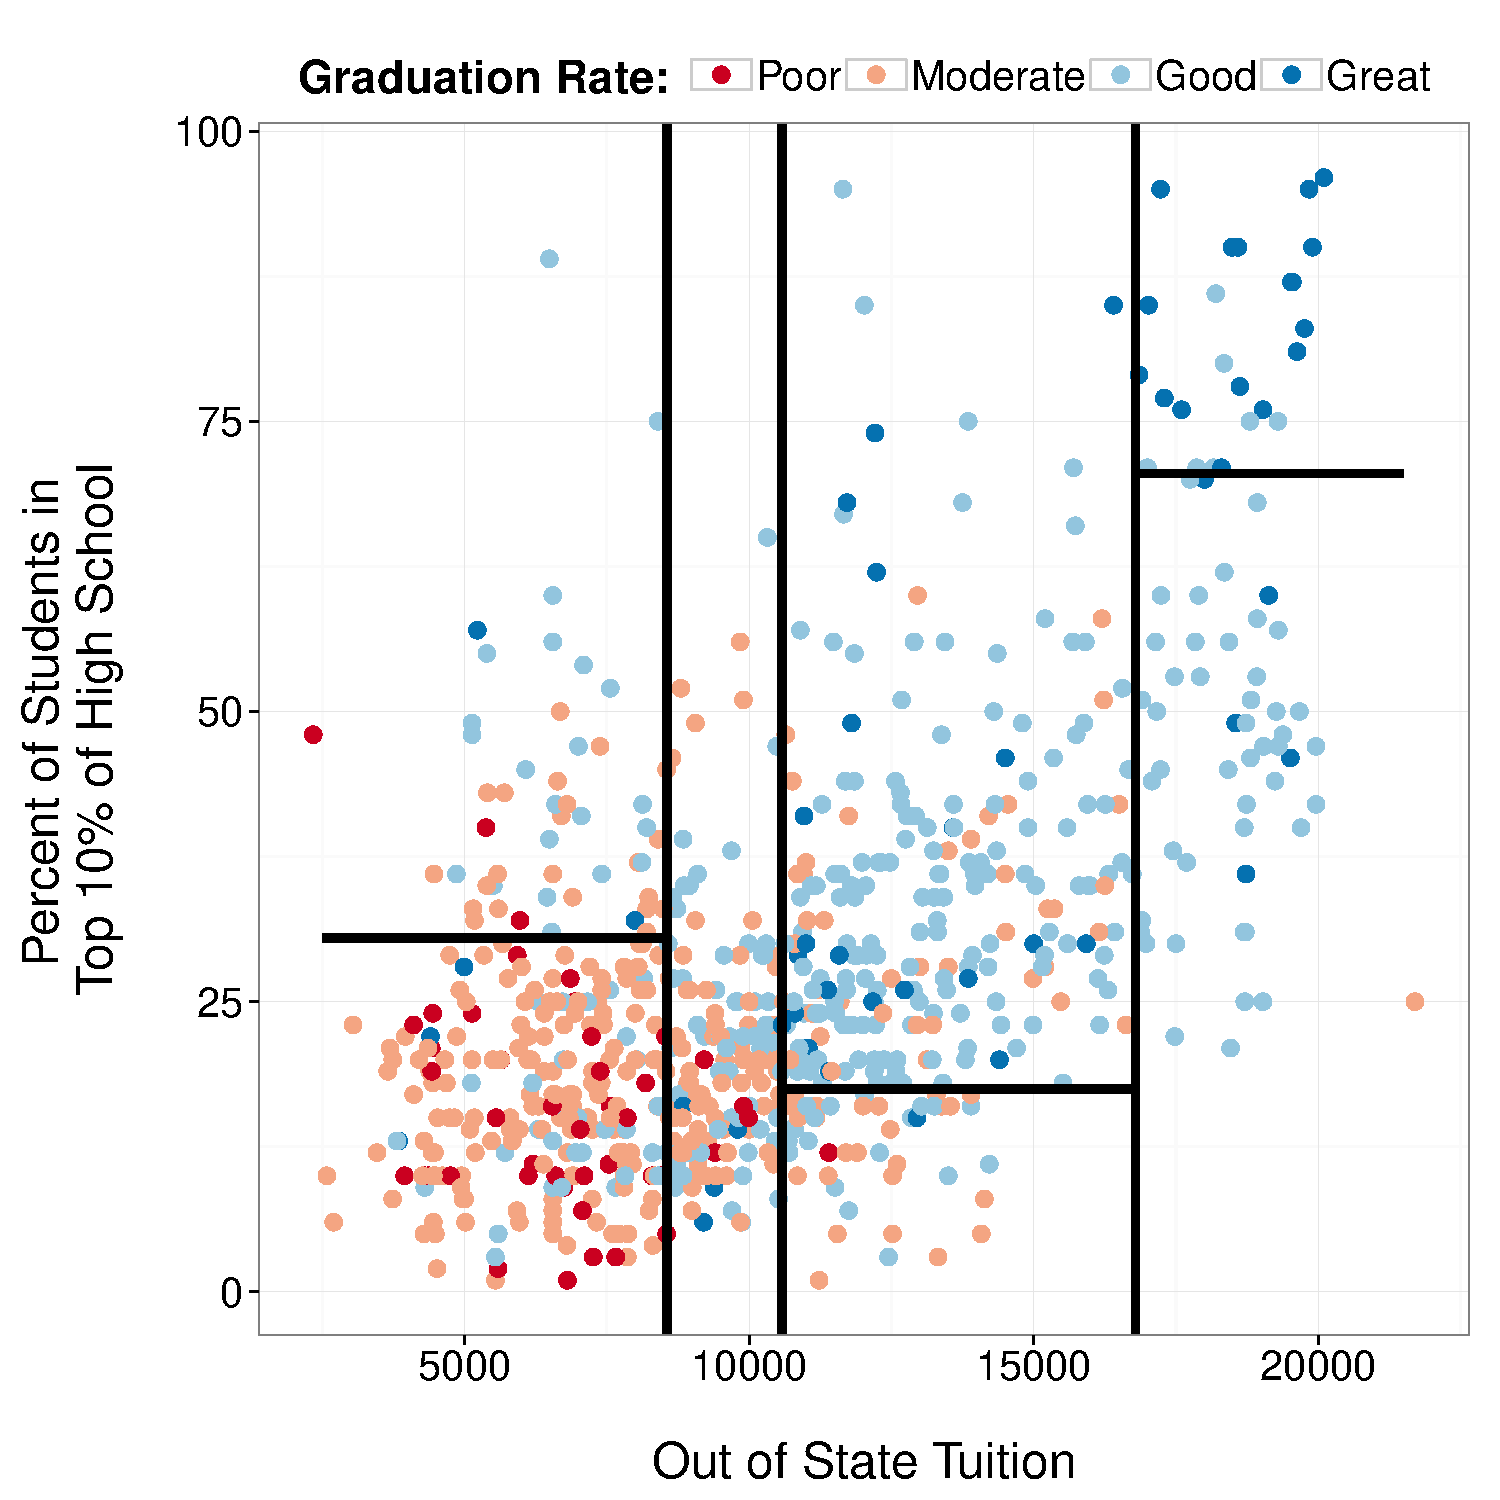
\includegraphics[width=\maxwidth]{figure/grad_rate_rpart_splits-1} 

\end{knitrout}

\end{center}

\columnbreak

\begin{center}

\begin{knitrout}
\definecolor{shadecolor}{rgb}{0.969, 0.969, 0.969}\color{fgcolor}
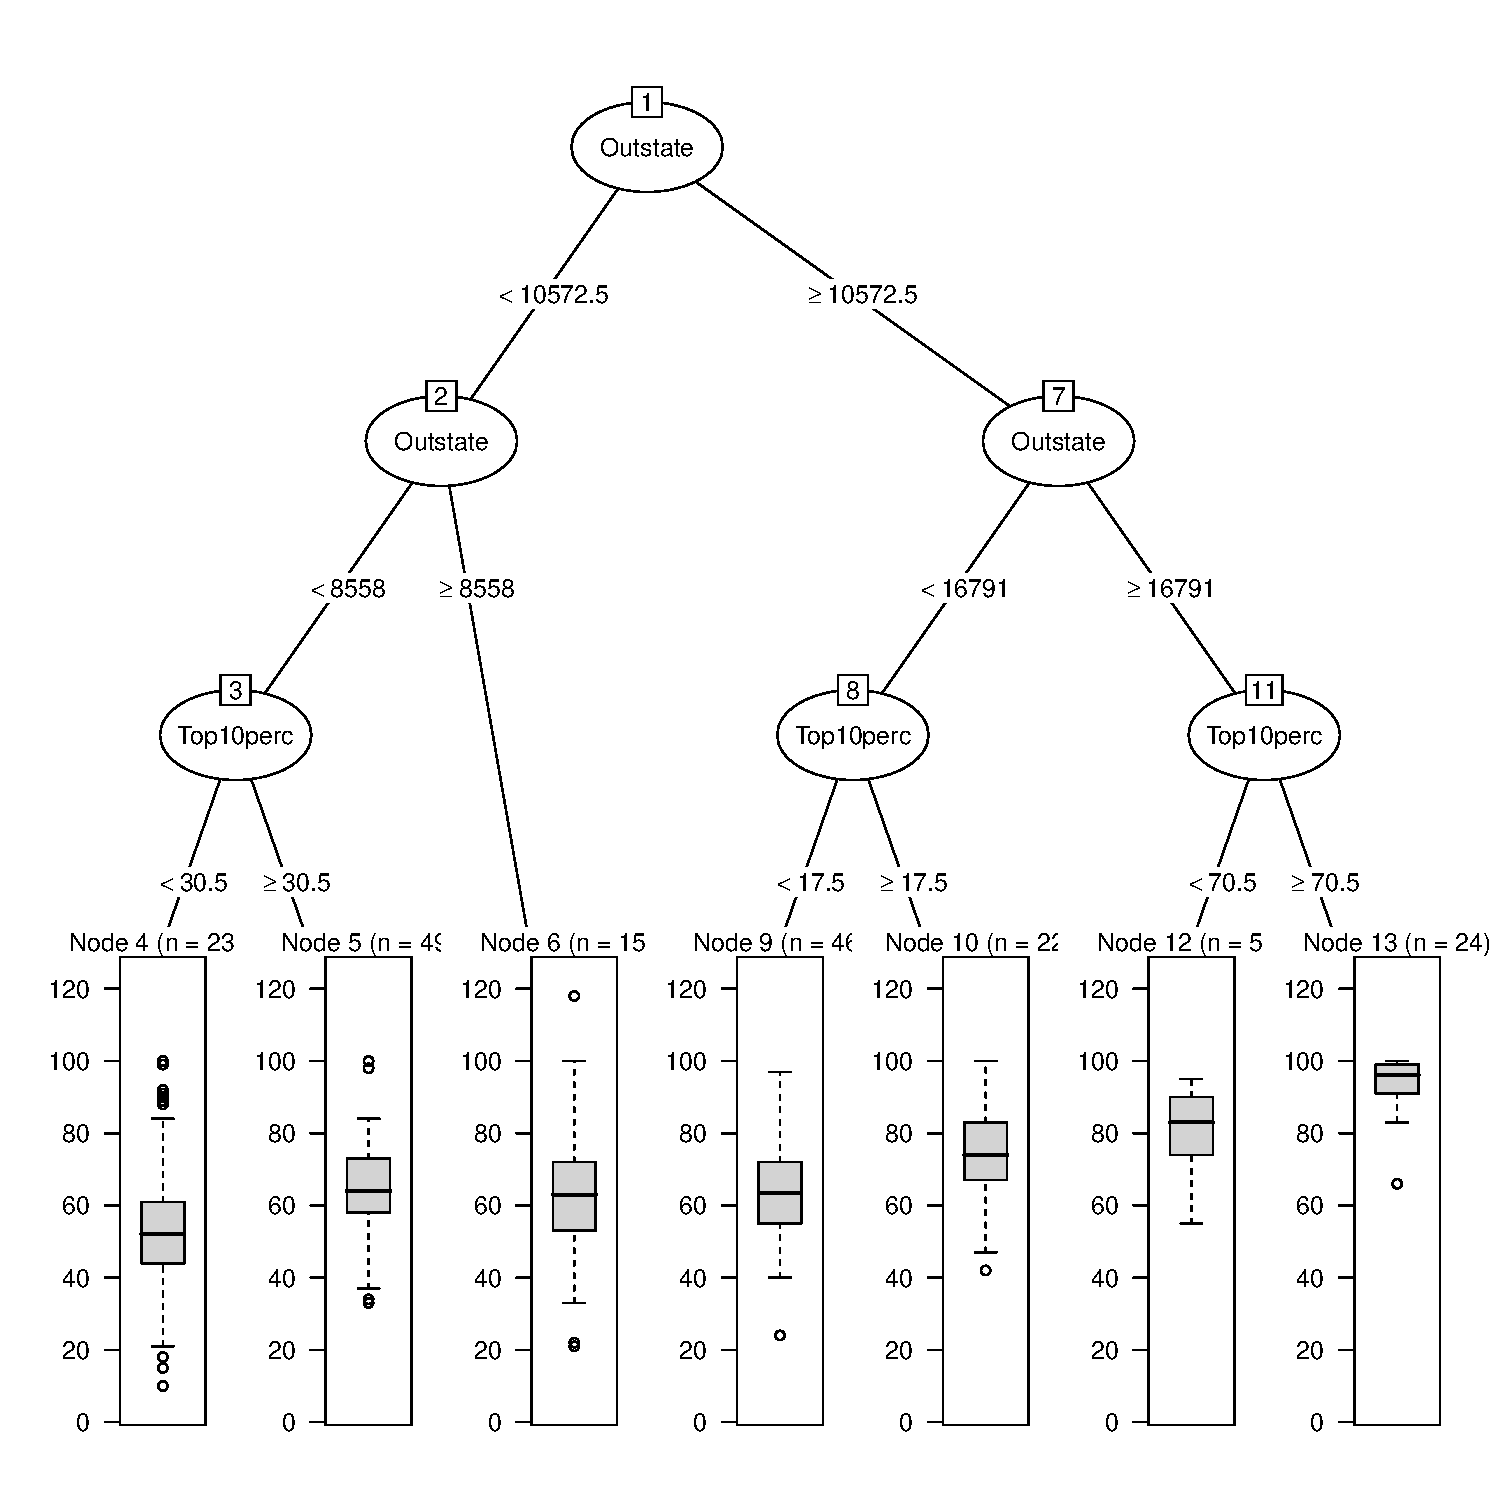
\includegraphics[width=\maxwidth]{figure/grad_rate_rpart_tree-1} 

\end{knitrout}

\end{center}

\end{multicols}

\end{frame}

%%%%%%%%%%%%%%%%%%%%%%%%%%%%%%%%%%%%%%%%%%%%%%%%%

\begin{frame}
\frametitle{Detour: The Bias-Variance Tradeoff}
\framesubtitle{training, testing, and cross-validation}

\begin{center}
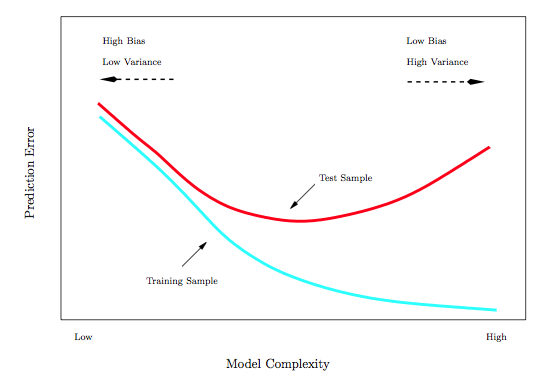
\includegraphics[width = 3.5in]{figure/bias_variance_tradeoff.png}
\end{center}
\scriptsize Source: \textit{An Introduction to Statistical Learning}

\end{frame}

%%%%%%%%%%%%%%%%%%%%%%%%%%%%%%%%%%%%%%%%%%%%%%%%%

\begin{frame}
\frametitle{Detour: The Bias-Variance Tradeoff}
\framesubtitle{training, testing, and cross-validation}

\begin{center}
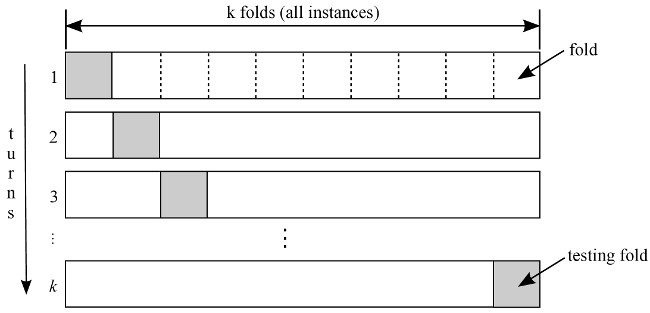
\includegraphics[width = 3.5in]{figure/k-fold-cross-validation.jpg}
\end{center}

\end{frame}

%%%%%%%%%%%%%%%%%%%%%%%%%%%%%%%%%%%%%%%%%%%%%%%%%

\begin{frame}
\frametitle{Decision Tree Pseudocode}

\textbf{CART: Breiman et al. (1984)}

\begin{enumerate}
\item Search all variables for splits in a greedy, top-down manner
\pause
\item Identify the best split by some criterion
\pause
\item Split the sample on this threshold, resulting in two child nodes
\pause
\item Repeat steps 1-3 on the resulting nodes until some stopping criterion is reached
\pause
\item Prune tree using cross-validation
\end{enumerate}

\end{frame}

%%%%%%%%%%%%%%%%%%%%%%%%%%%%%%%%%%%%%%%%%%%%%%%%%

\begin{frame}
\frametitle{Handling Missingness - Decision Trees}
\framesubtitle{surrogate splits}

\begin{center}
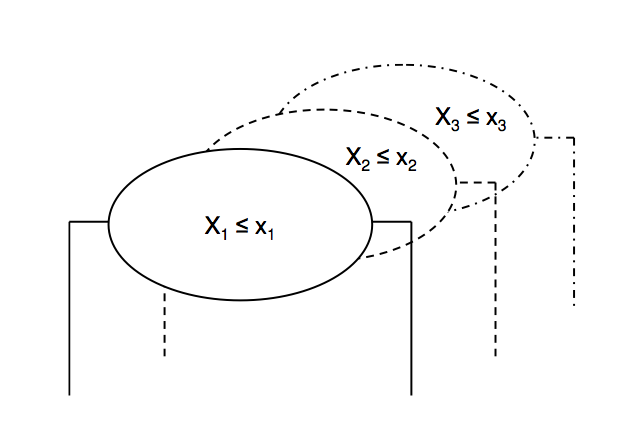
\includegraphics[width = 2.5in]{figure/surrogate_split.png}
\end{center}
\scriptsize Source: \textit{Hapfelmeier (2012)}

\end{frame}

%%%%%%%%%%%%%%%%%%%%%%%%%%%%%%%%%%%%%%%%%%%%%%%%%

\begin{frame}
\frametitle{Recap: Pros and Cons of Decision Trees}

\textbf{Pros:}
\begin{itemize}
\item intuitive, easy to explain and visualize
\item can handle continuous or categorical outcomes
\item non-parametric, robust to outliers
\item no model specification required
\end{itemize}

\vspace{3ex}

\pause

\textbf{Cons:}
\begin{itemize}
\item biased toward variables with many possible splits
\item typically outperformed by regression techniques
\item prone to overfitting
\end{itemize}

\end{frame}

%%%%%%%%%%%%%%%%%%%%%%%%%%%%%%%%%%%%%%%%%%%%%%%%%

\begin{frame}
\frametitle{Random Forest Pseudocode}

\textbf{CART forests: Breiman (2001)}

\begin{enumerate}
\item Take a bootstrap sample
\pause
\item Select a random subset of predictors
\pause
\item Fit a decision tree to full depth
\pause
\item Repeat 500ish times
\end{enumerate}

\end{frame}

%%%%%%%%%%%%%%%%%%%%%%%%%%%%%%%%%%%%%%%%%%%%%%%%%

\begin{frame}
\frametitle{Creating Ensembles of Trees}



\begin{multicols}{2}

\begin{center}

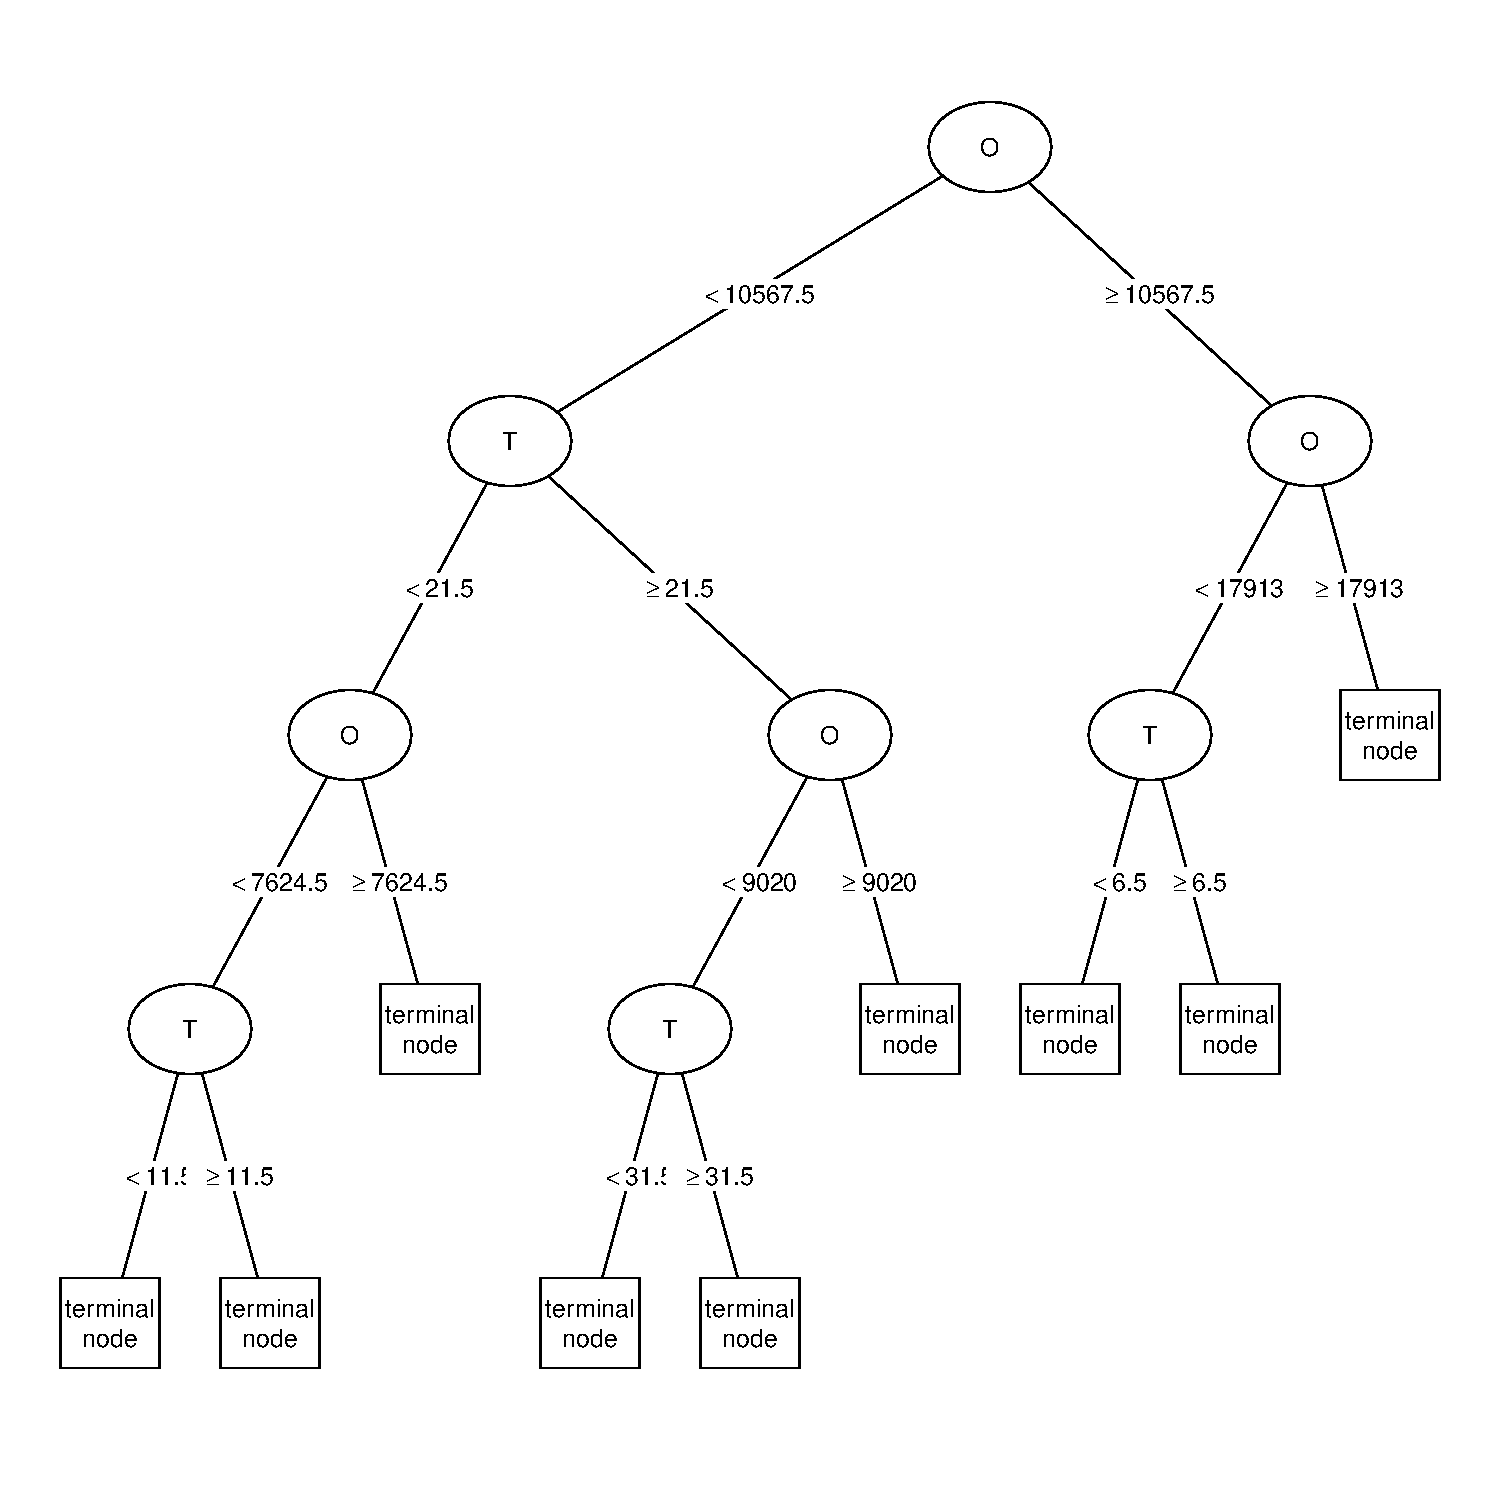
\includegraphics[width = 1.3in]{figure/boot_tree_1.pdf} \\
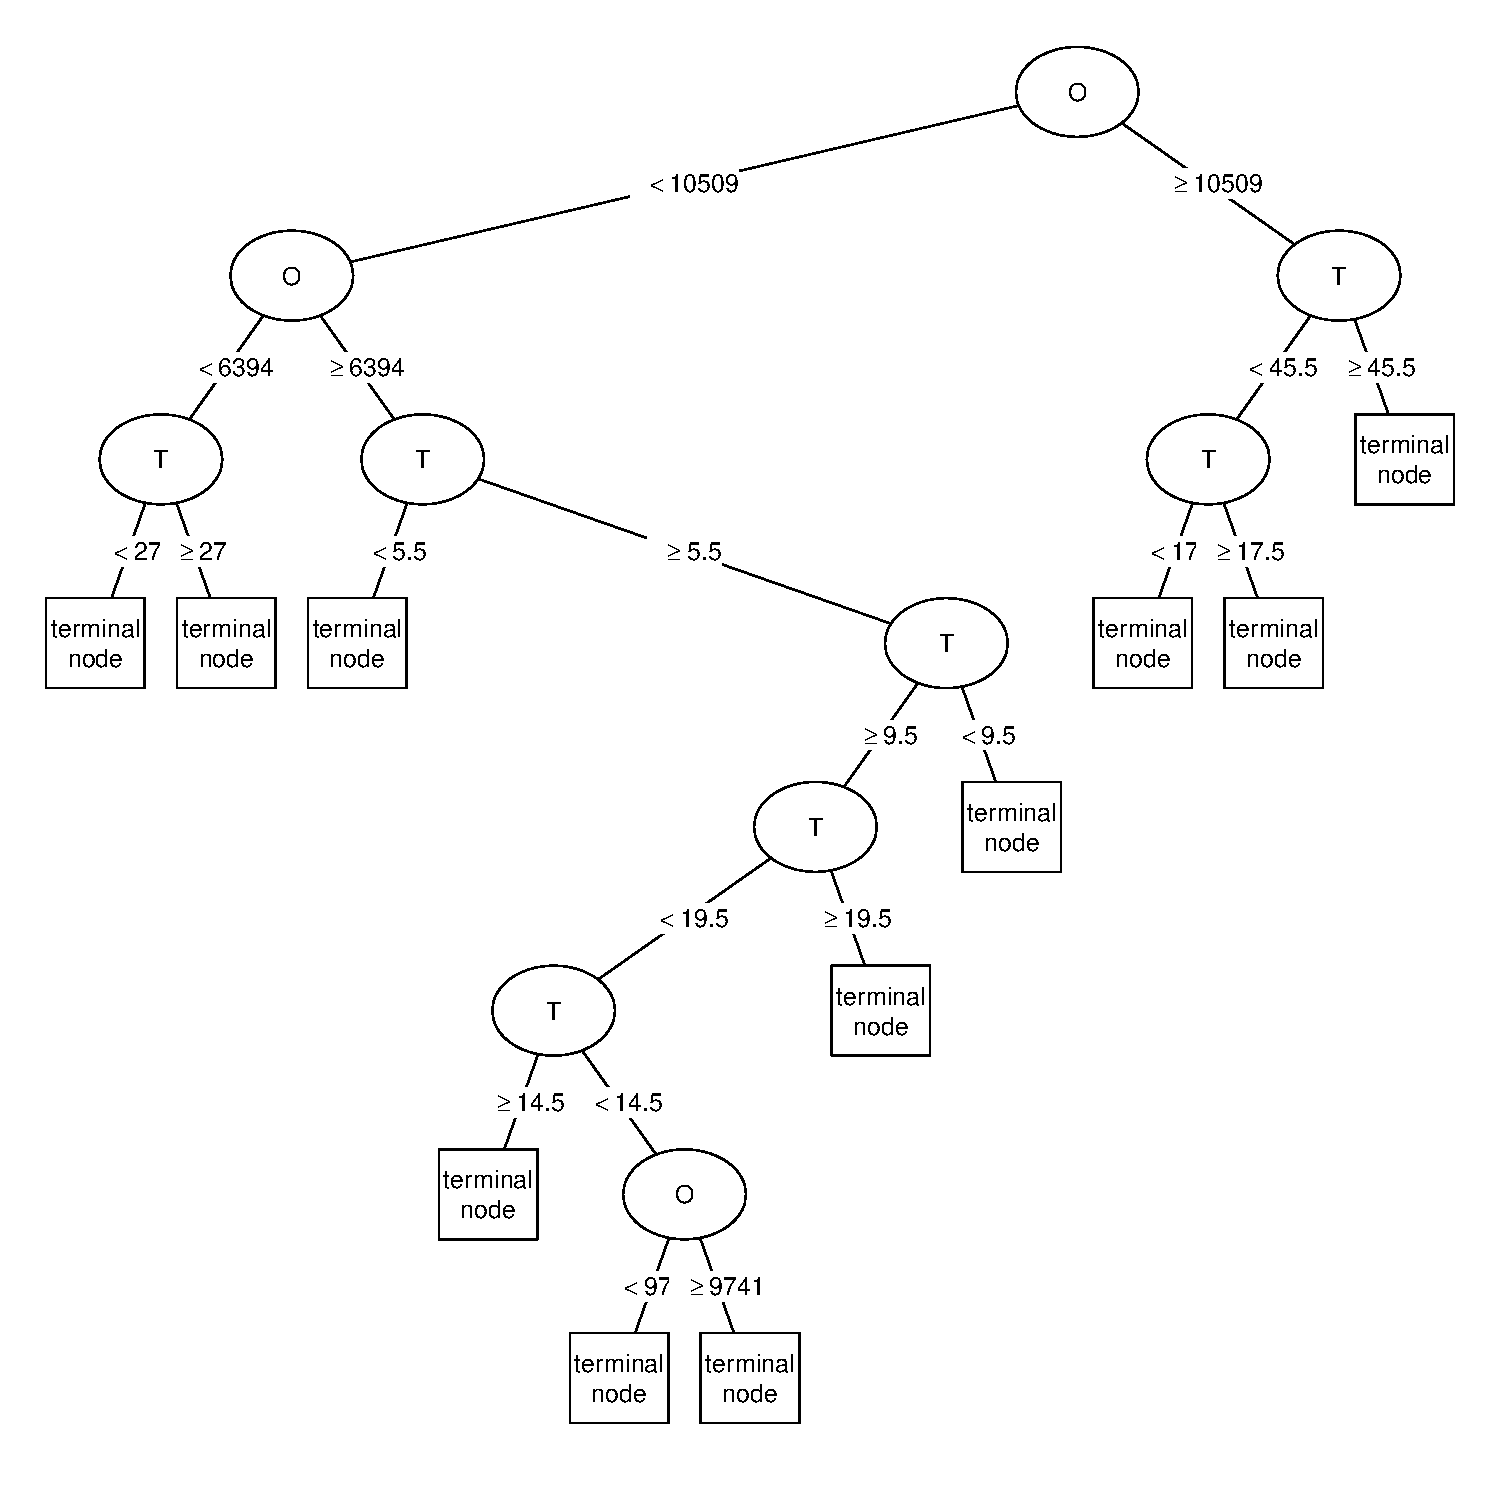
\includegraphics[width = 1.3in]{figure/boot_tree_2.pdf}

\end{center}

\columnbreak

\begin{center}

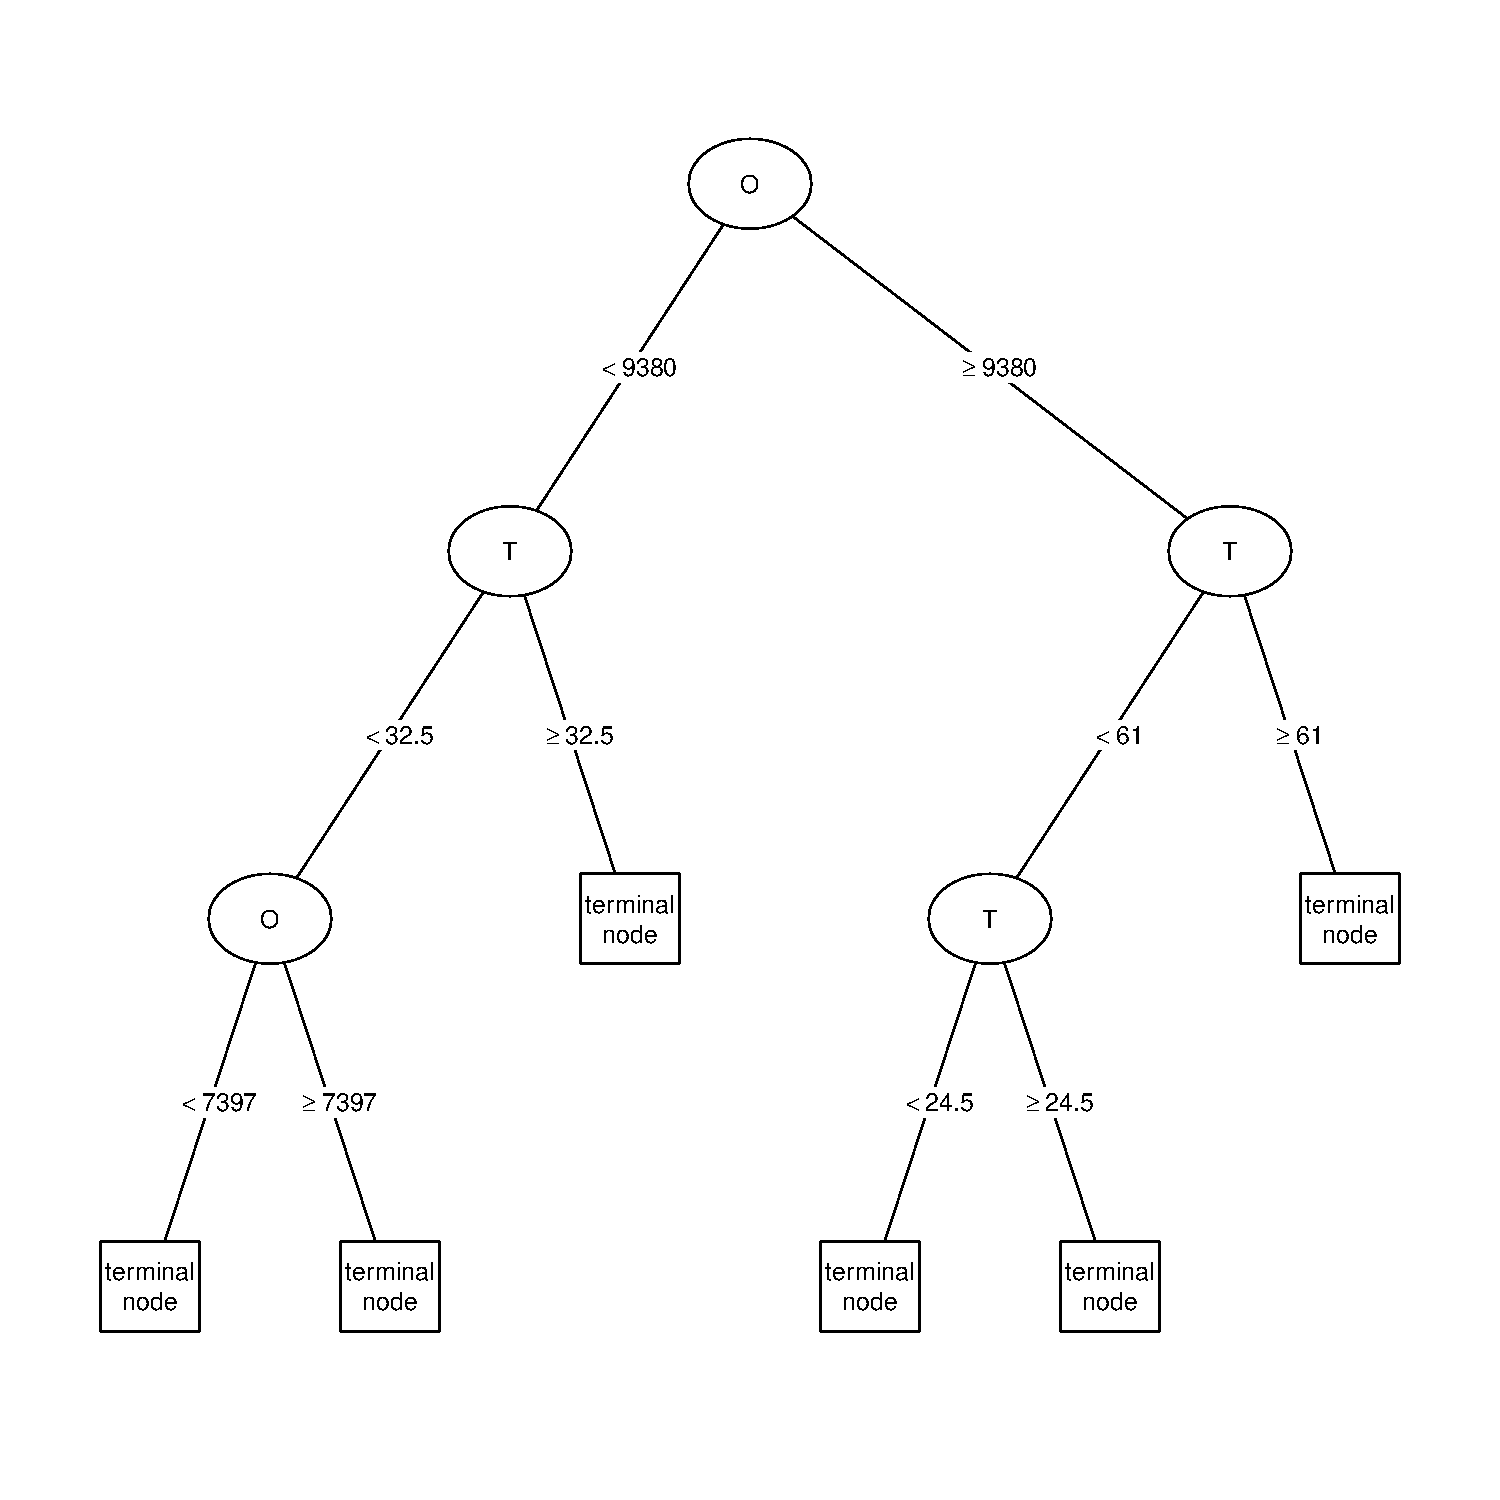
\includegraphics[width = 1.3in]{figure/boot_tree_3.pdf} \\
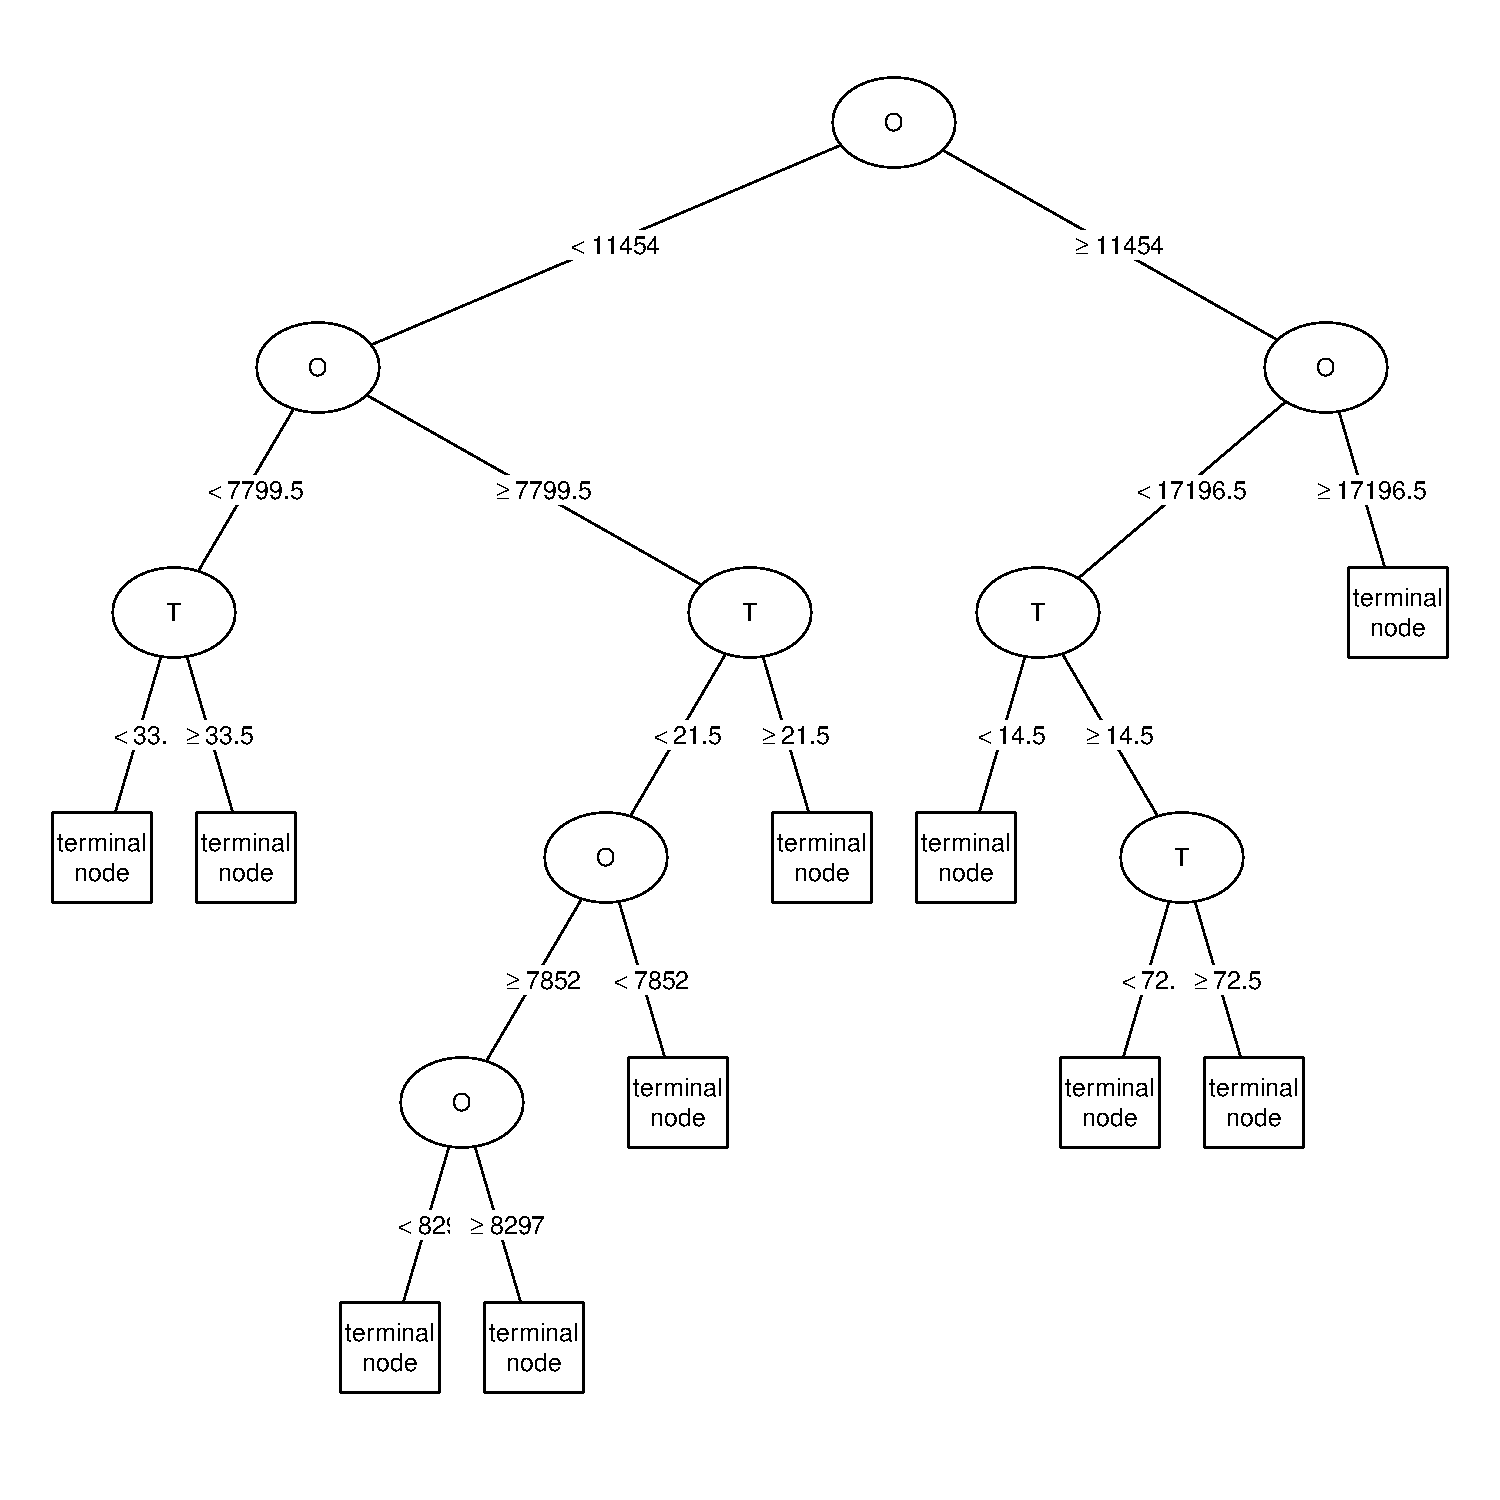
\includegraphics[width = 1.3in]{figure/boot_tree_4.pdf}

\end{center}

\end{multicols}

\end{frame}

%%%%%%%%%%%%%%%%%%%%%%%%%%%%%%%%%%%%%%%%%%%%%%%%%

\begin{frame}
\frametitle{Creating Ensembles of Trees}
\framesubtitle{why it works - theoretical}

\begin{center}
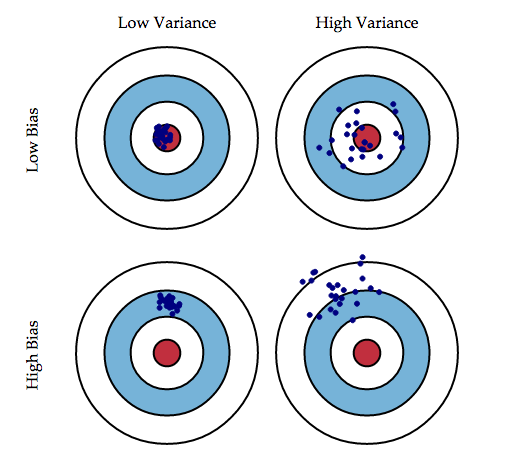
\includegraphics[width = 2.5in]{figure/bias_var_target.png}
\end{center}
\scriptsize Source: \textit{Scott Fortmann-Roe}

\end{frame}

%%%%%%%%%%%%%%%%%%%%%%%%%%%%%%%%%%%%%%%%%%%%%%%%%

\begin{frame}
\frametitle{Creating Ensembles of Trees}
\framesubtitle{why it works - applied}

\begin{center}
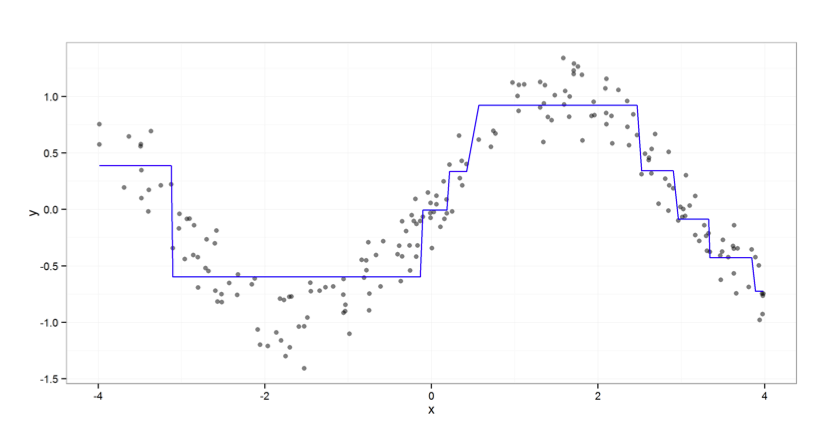
\includegraphics[width = 3.5in]{figure/cart_sin_curve.png}
\end{center}
\scriptsize Source: \textit{Zachary Jones}

\end{frame}

%%%%%%%%%%%%%%%%%%%%%%%%%%%%%%%%%%%%%%%%%%%%%%%%%

\begin{frame}
\frametitle{Creating Ensembles of Trees}
\framesubtitle{why it works - applied}

\begin{center}
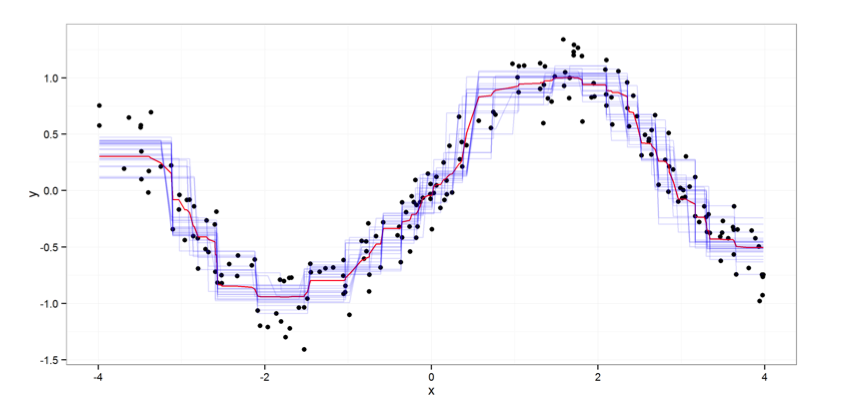
\includegraphics[width = 3.5in]{figure/forest_sin_curve.png}
\end{center}
\scriptsize Source: \textit{Zachary Jones}

\end{frame}

%%%%%%%%%%%%%%%%%%%%%%%%%%%%%%%%%%%%%%%%%%%%%%%%%

\begin{frame}
\frametitle{Handling Missingness - Forests}
\framesubtitle{imputation by proximity}

For missing data:

\begin{enumerate}
\item Calculate proximity matrix (number of times observations show up in the same node)
\item Impute missing values using medians and levels of the highest frequency
\item Run a random forest model
\item Update missing values to a weighted mean of the observations or category with the largest average proximity
\item Repeat 5-10 times
\end{enumerate}

\end{frame}

%%%%%%%%%%%%%%%%%%%%%%%%%%%%%%%%%%%%%%%%%%%%%%%%%

\begin{frame}
\frametitle{Recap: Pros and Cons of Decision Trees}

\textbf{Pros:}
\begin{itemize}
\item All the CART pros!
\item Can now approximate smooth, nonlinear relationships instead of piecewise constant fits
\item Unlikely to overfit
\item Not much tuning required compared to other algorithmic methods
\end{itemize}

\vspace{3ex}

\pause

\textbf{Cons:}
\begin{itemize}
\item still biased toward variables with many possible splits
\item Harder to interpret
\item Longer computation time (still manageable for large datasets)
\end{itemize}

\end{frame}

%%%%%%%%%%%%%%%%%%%%%%%%%%%%%%%%%%%%%%%%%%%%%%%%%

\begin{frame}
\frametitle{Interpreting the Black Box}

\begin{enumerate}
\item Variable Importance
\item Partial Dependence Plots
\end{enumerate}

\pause

\vspace{3ex}

more on this in a sec...

\end{frame}

%%%%%%%%%%%%%%%%%%%%%%%%%%%%%%%%%%%%%%%%%%%%%%%%%

\begin{frame}
\frametitle{Not a ``Magic'' Solution}

\begin{multicols}{2}

\begin{center}
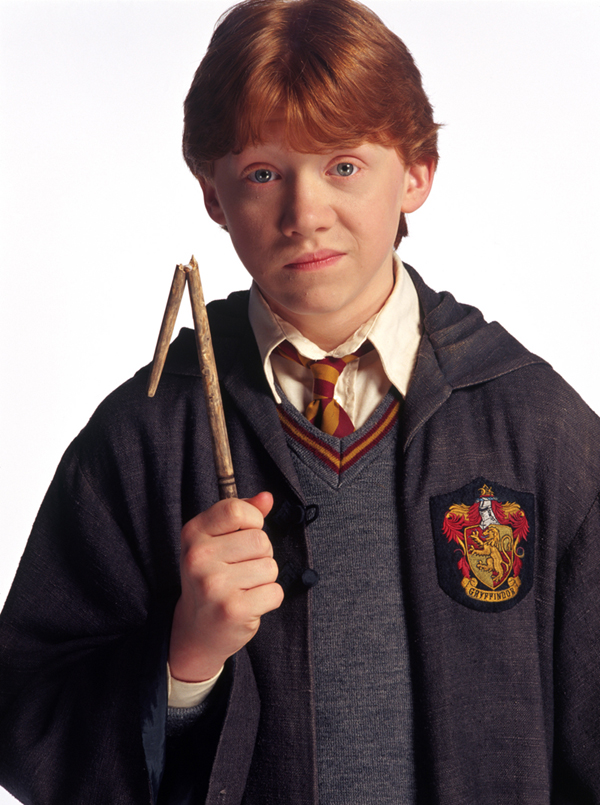
\includegraphics[height = 2.2in]{figure/magic_wand.jpg}
\end{center}

\columnbreak

\pause

\vspace{3ex}

Random forests make no general assumptions regarding independence, and thus have the potential to be used for multilevel EDA with \textbf{little added complexity}

\pause

\vspace{3ex}

However, not much is known about what happens when forests are used in this way

\end{multicols}

\end{frame}

%%%%%%%%%%%%%%%%%%%%%%%%%%%%%%%%%%%%%%%%%%%%%%%%%

\section{Multilevel Extensions}
\begin{frame}
\frametitle{Proof of Concept}

\begin{knitrout}
\definecolor{shadecolor}{rgb}{0.969, 0.969, 0.969}\color{fgcolor}
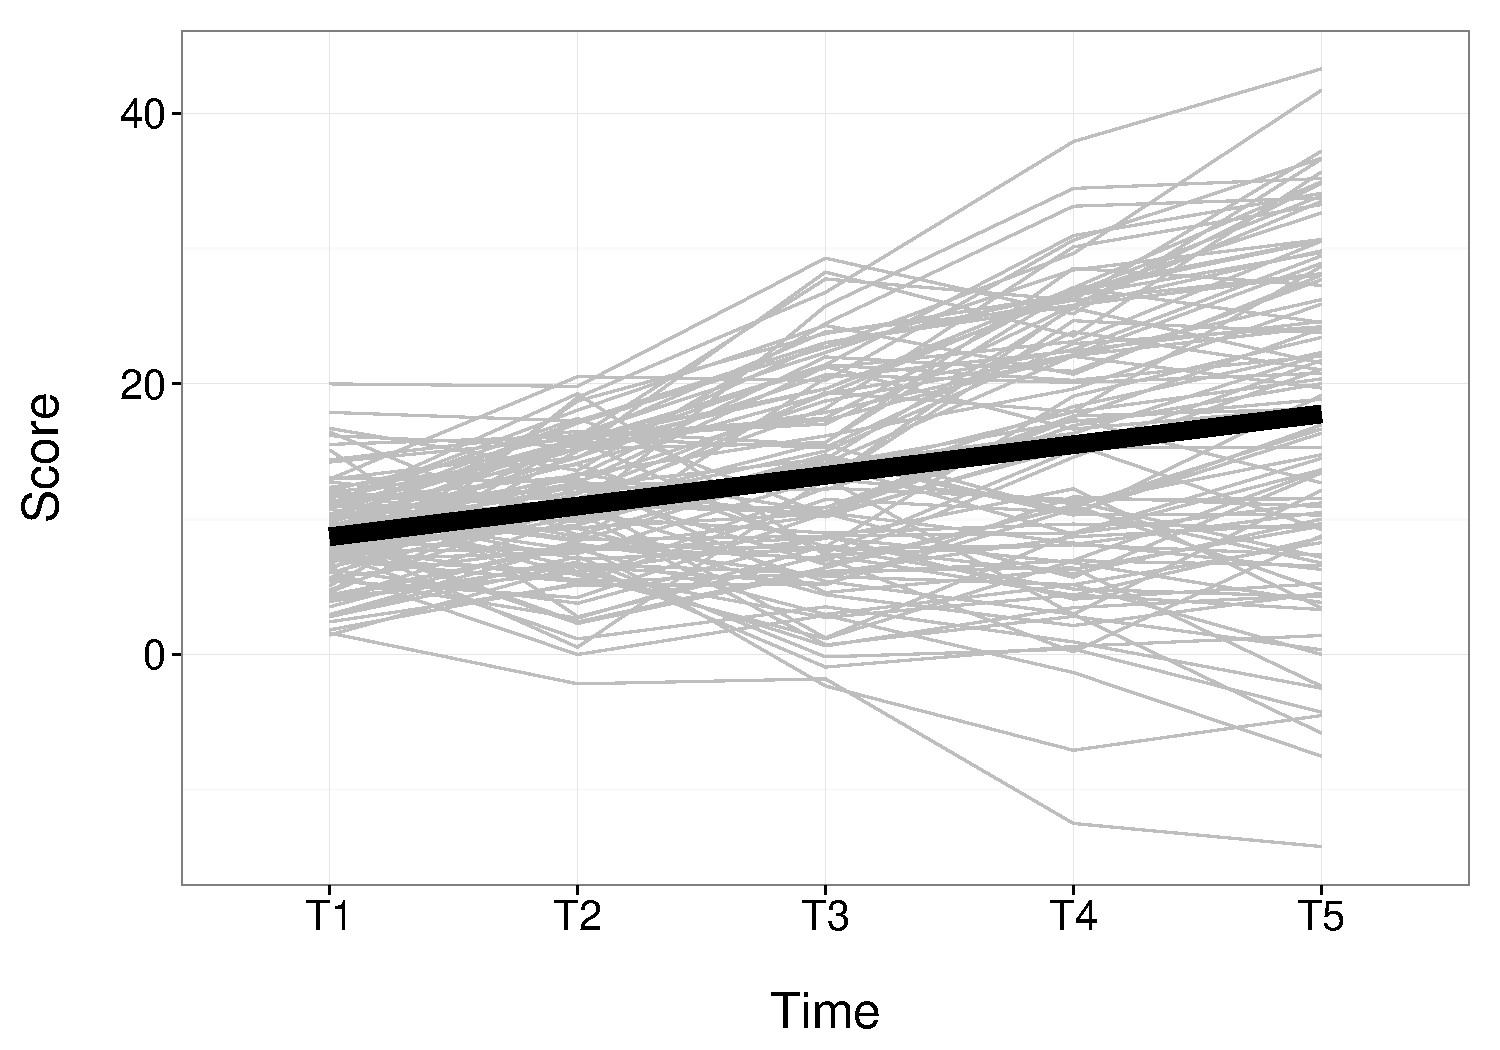
\includegraphics[width=\maxwidth]{figure/longData-1} 

\end{knitrout}

\end{frame}

%%%%%%%%%%%%%%%%%%%%%%%%%%%%%%%%%%%%%%%%%%%%%%%%%

\begin{frame}
\frametitle{Proof of Concept}

\begin{knitrout}
\definecolor{shadecolor}{rgb}{0.969, 0.969, 0.969}\color{fgcolor}
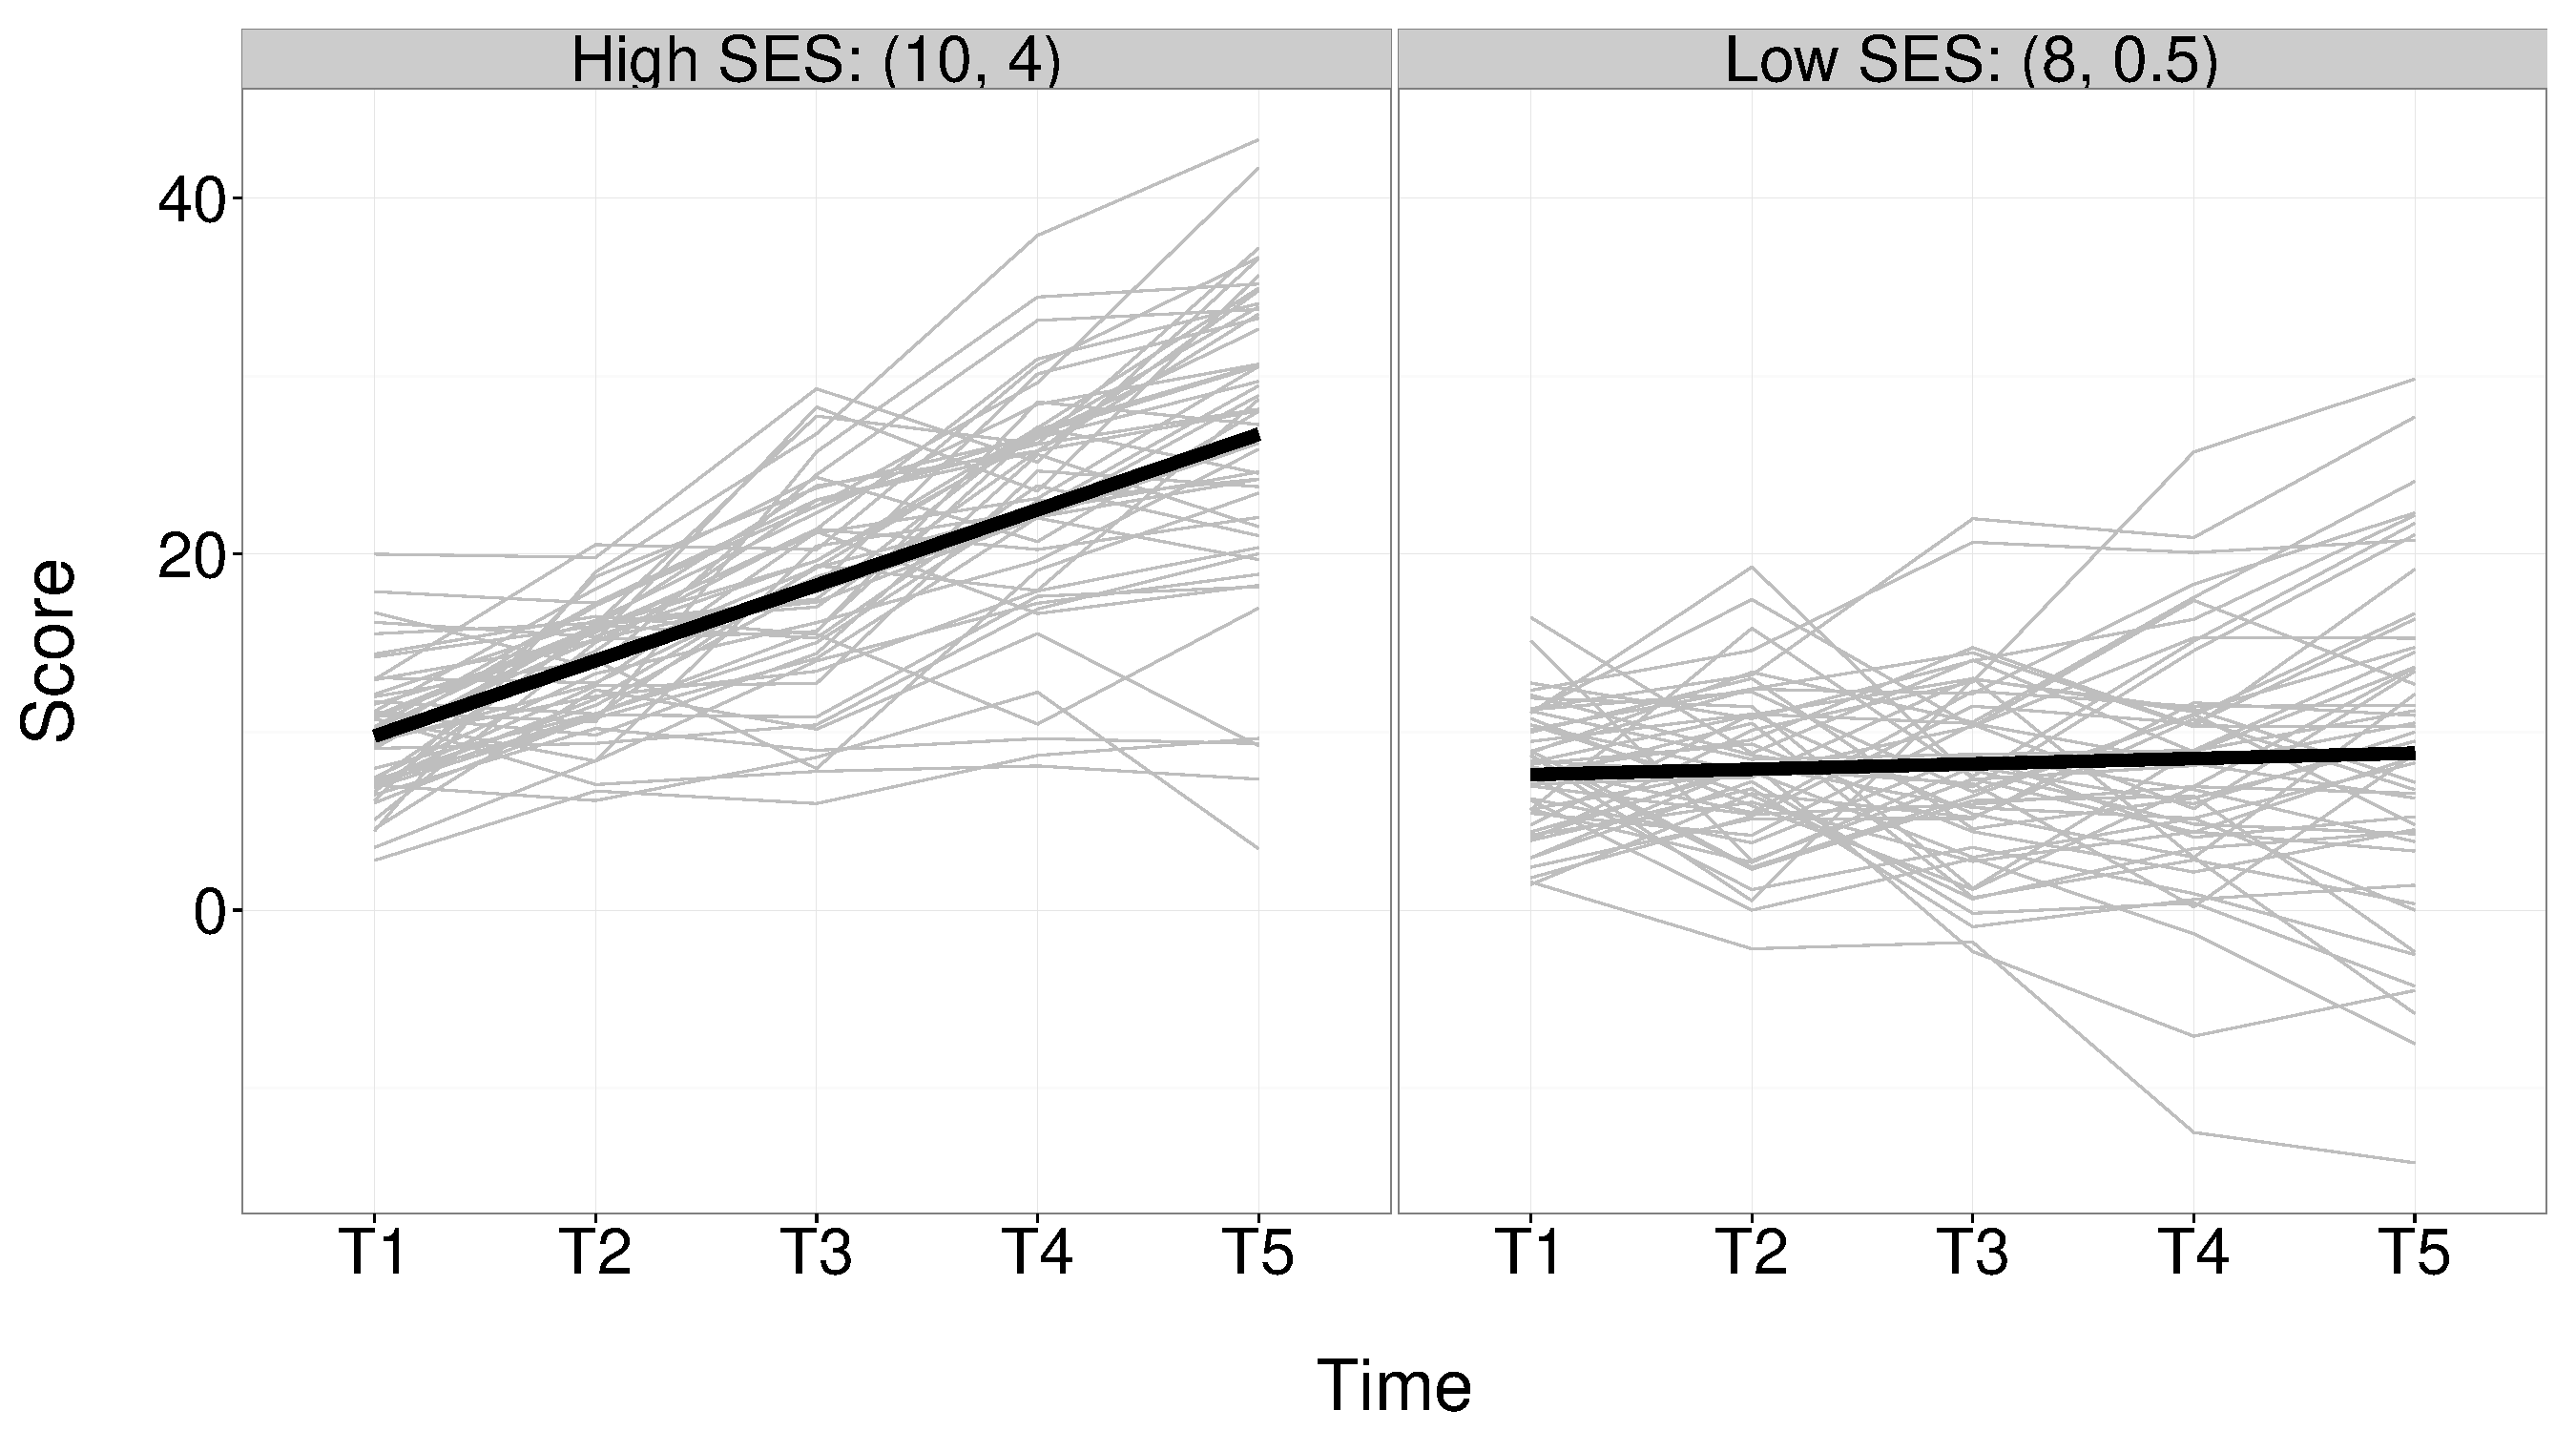
\includegraphics[width=\maxwidth]{figure/longDataSub-1} 

\end{knitrout}

\end{frame}

%%%%%%%%%%%%%%%%%%%%%%%%%%%%%%%%%%%%%%%%%%%%%%%%%

\begin{frame}
\frametitle{Proof of Concept}

\begin{knitrout}
\definecolor{shadecolor}{rgb}{0.969, 0.969, 0.969}\color{fgcolor}
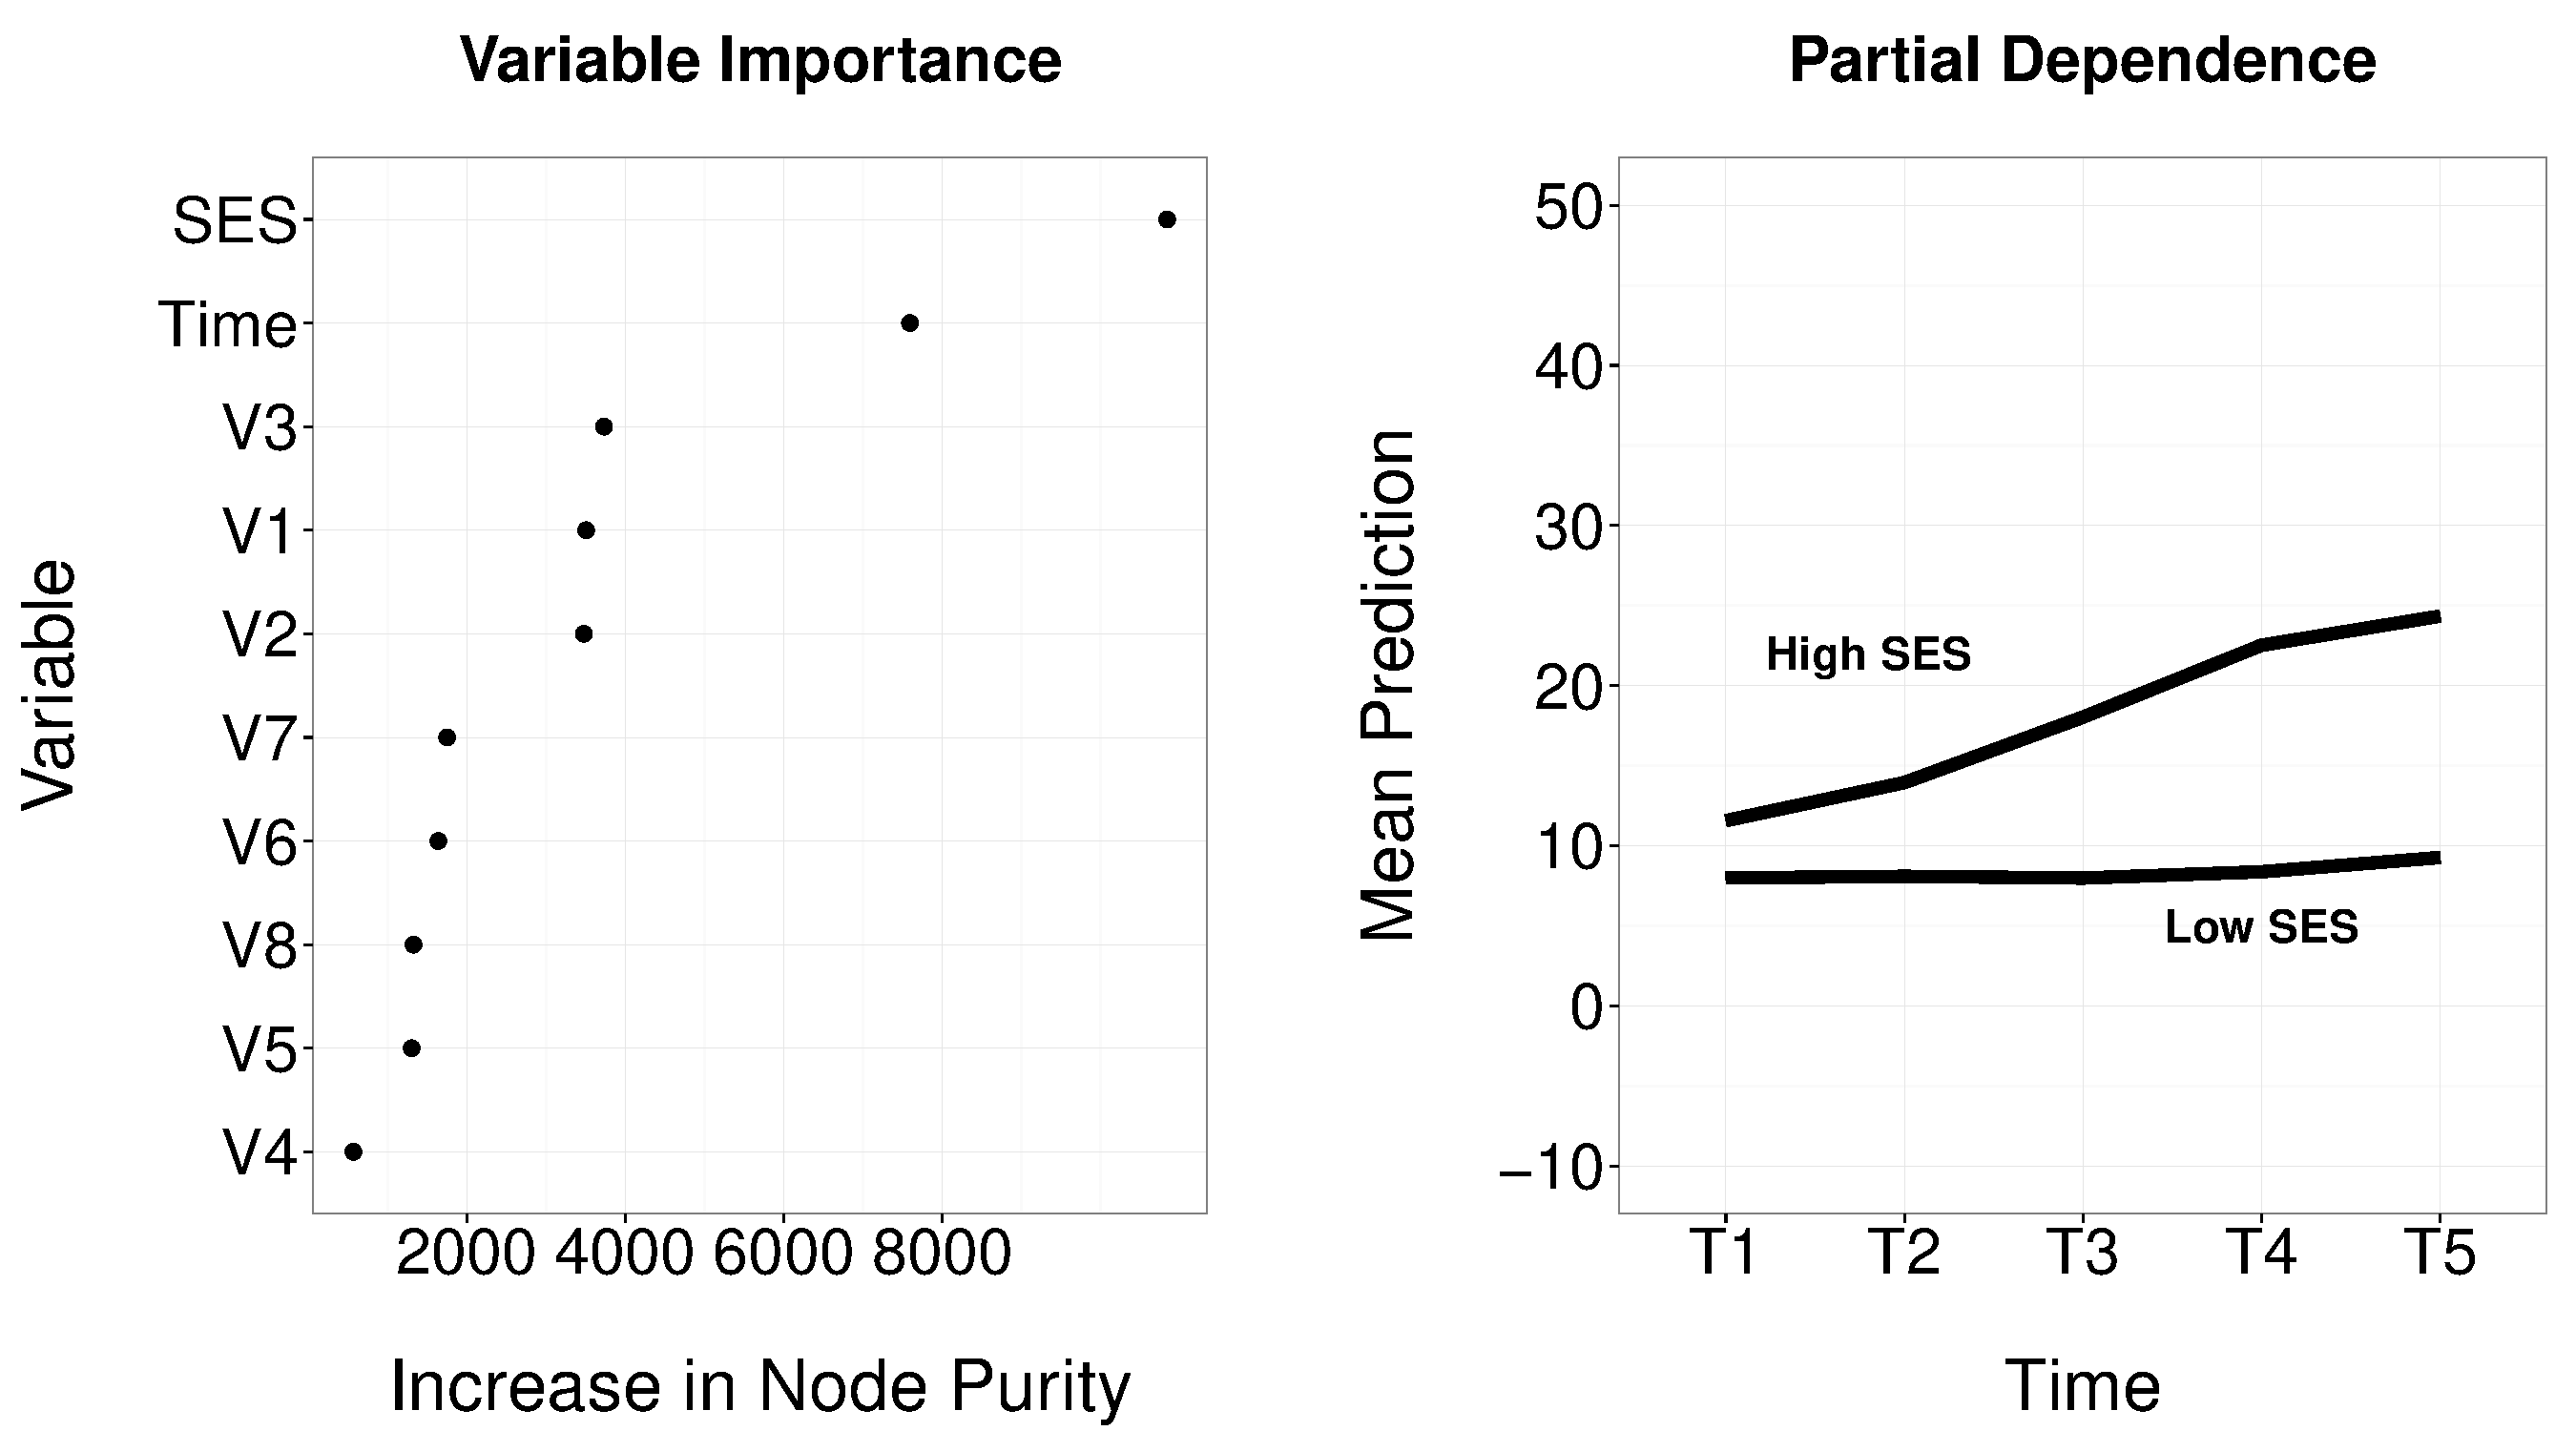
\includegraphics[width=\maxwidth]{figure/longDataResults-1} 

\end{knitrout}

\end{frame}

%%%%%%%%%%%%%%%%%%%%%%%%%%%%%%%%%%%%%%%%%%%%%%%%%

\section{Multilevel Issues}
\begin{frame}
\frametitle{Issue 1: CART biased variable selection}
\framesubtitle{single level (N = 1000)}

\begin{knitrout}
\definecolor{shadecolor}{rgb}{0.969, 0.969, 0.969}\color{fgcolor}
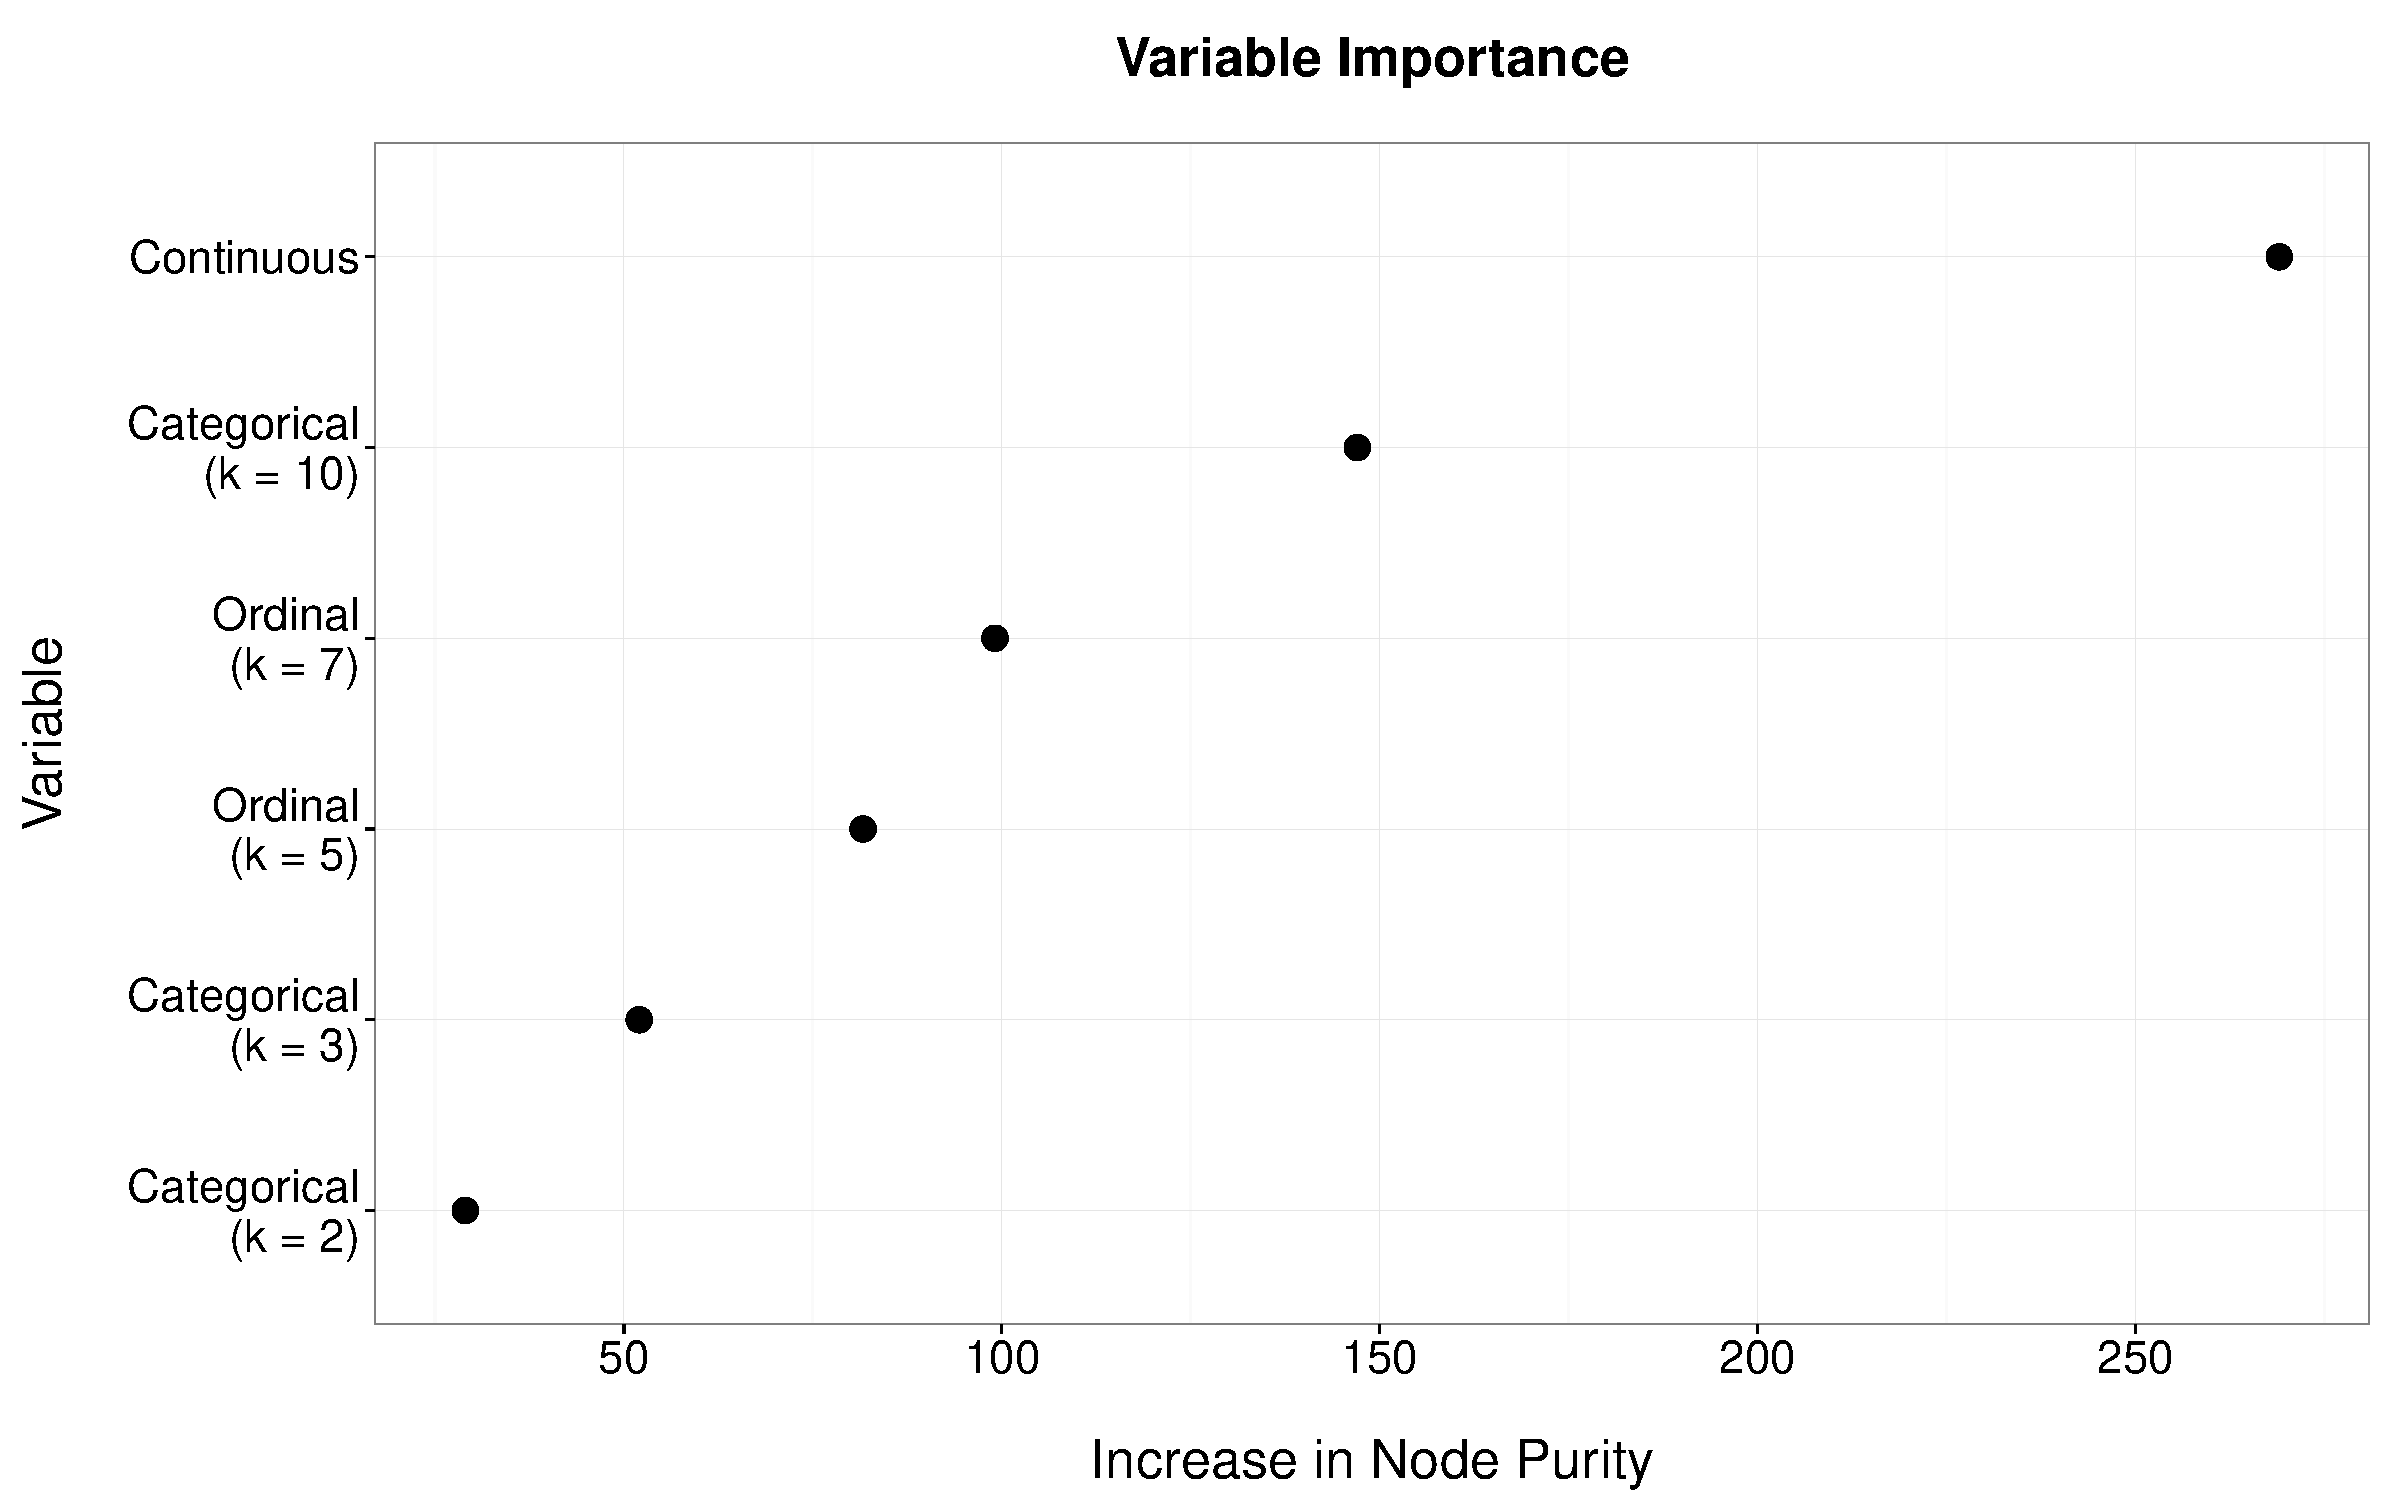
\includegraphics[width=\maxwidth]{figure/bias_importance_lev1-1} 

\end{knitrout}

\end{frame}

%%%%%%%%%%%%%%%%%%%%%%%%%%%%%%%%%%%%%%%%%%%%%%%%%

\begin{frame}
\frametitle{Issue 1: CART biased variable selection}
\framesubtitle{multilevel (N = 1000, L2/L1 = 100/10)}

\begin{knitrout}
\definecolor{shadecolor}{rgb}{0.969, 0.969, 0.969}\color{fgcolor}
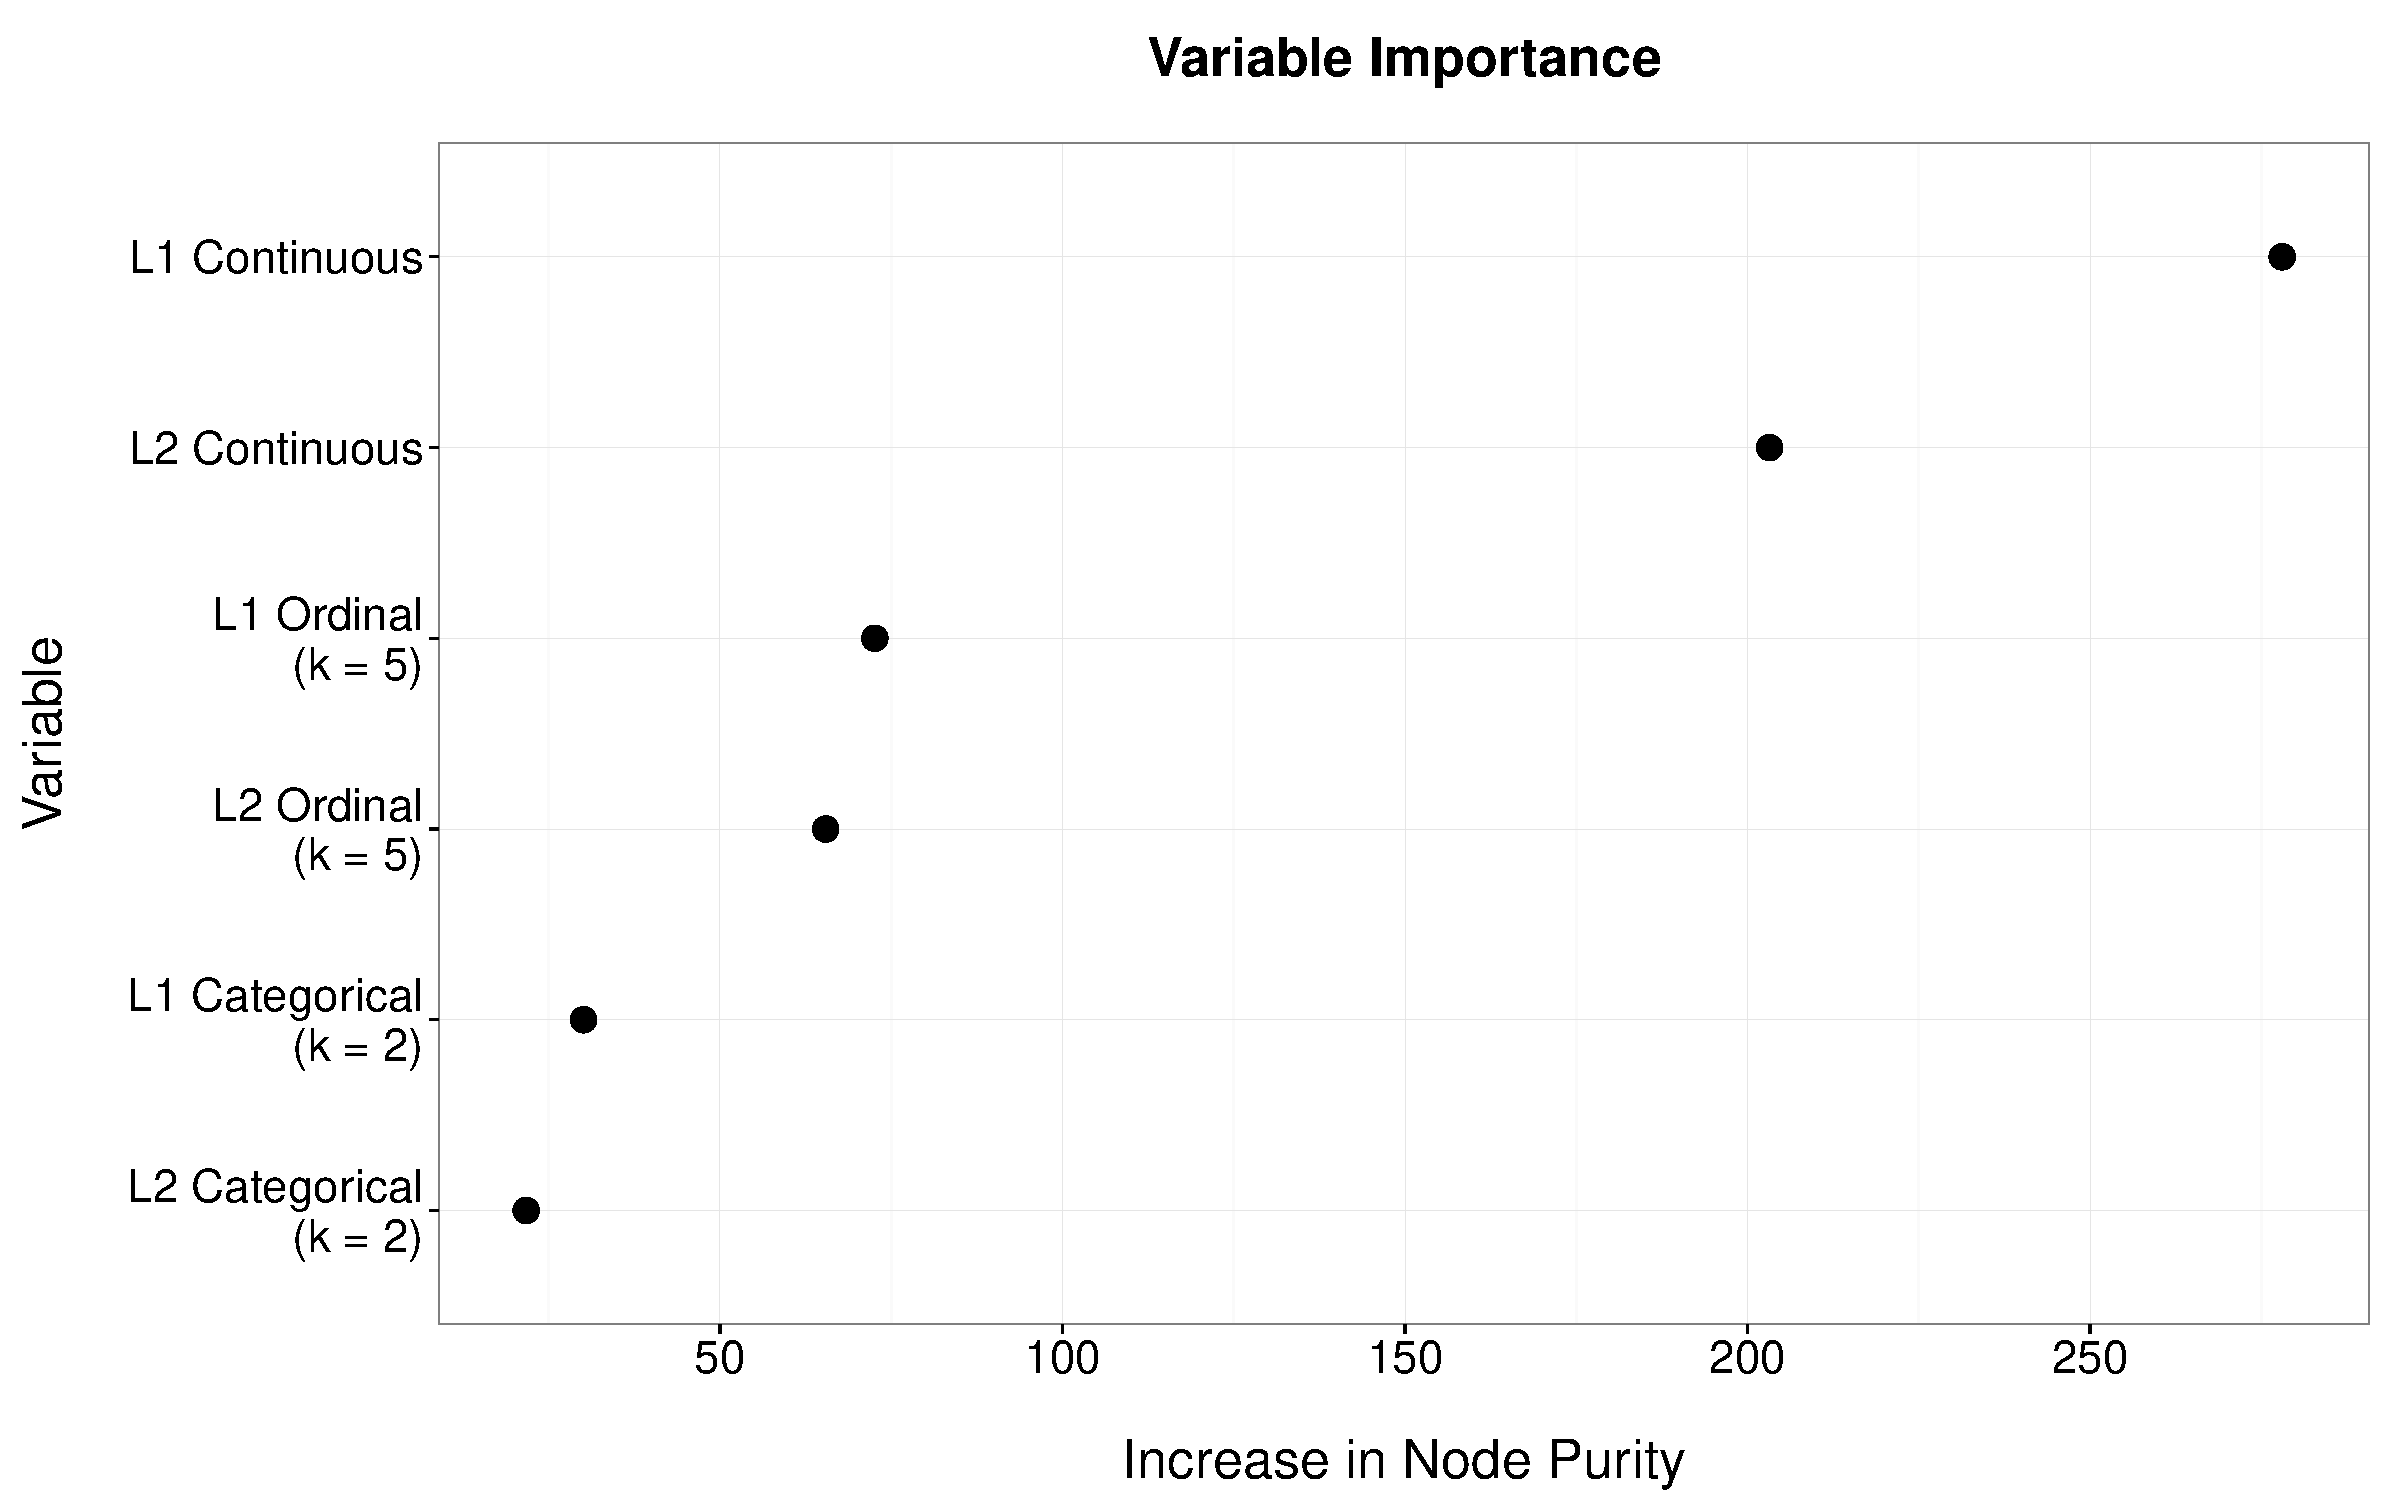
\includegraphics[width=\maxwidth]{figure/bias_importance_lev2-1} 

\end{knitrout}

\end{frame}

%%%%%%%%%%%%%%%%%%%%%%%%%%%%%%%%%%%%%%%%%%%%%%%%%

\begin{frame}
\frametitle{Issue 2: Underestimation of OOB error}

\begin{multicols}{2}

\begin{center}
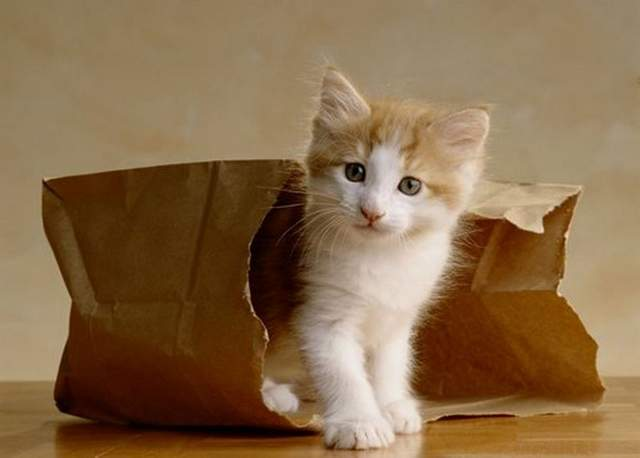
\includegraphics[width = 2in]{figure/oob.jpg}
\end{center}

\columnbreak

\begin{center}

$P_{notselected} = (1 - \frac{1}{n})^n$

\vspace{3ex}

$\lim_{n\to\infty} P = \frac{1}{e} \approx 0.368$

\end{center}

\end{multicols}

\end{frame}

%%%%%%%%%%%%%%%%%%%%%%%%%%%%%%%%%%%%%%%%%%%%%%%%%

\begin{frame}
\frametitle{Issue 2: Underestimation of OOB error}



\begin{multicols}{2}

\begin{center}
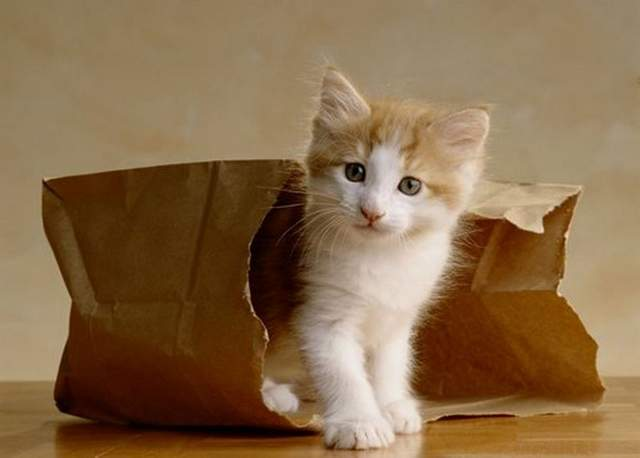
\includegraphics[width = 2in]{figure/oob.jpg}
\end{center}

\columnbreak

\begin{center}

$MSE_{test}$ = $48.32$ 

\vspace{3ex}

$MSE_{OOB}$ = $23.95$

\end{center}

\end{multicols}

\end{frame}

%%%%%%%%%%%%%%%%%%%%%%%%%%%%%%%%%%%%%%%%%%%%%%%%%

\begin{frame}
\frametitle{Reminder: Issues to Keep in Mind}

\begin{itemize}
\item OOB errer estimates will be unreliable
\item Additional bias for level-2 variables occurs
\item DO NOT use this method and then perform confirmatory tests on the same data
\end{itemize}

\end{frame}

%%%%%%%%%%%%%%%%%%%%%%%%%%%%%%%%%%%%%%%%%%%%%%%%%

\begin{frame}
\frametitle{Analysis Steps}

\begin{enumerate}
\item Initial pre-processing (``feature engineering'', handle missingness)
\item Estimate ICC and consider what level the variables were measured at
\item Estimate predictive performance using a hold out test set or cross-validation (at level-2)
\item Examine variable importance and partial dependence plots
\end{enumerate}

\end{frame}

%%%%%%%%%%%%%%%%%%%%%%%%%%%%%%%%%%%%%%%%%%%%%%%%%

\begin{frame}
\frametitle{Helpful (and Accessible) Citations}

Breiman, L. (2001). Statistical modeling: The two cultures \\

Shmueli, G. (2010). To explain or predict? \\

Strobl, C. et al. (2009). An introduction to recursive partitioning: rationale, application, and characteristics of classification and regression trees, bagging, and random forests

\end{frame}

%%%%%%%%%%%%%%%%%%%%%%%%%%%%%%%%%%%%%%%%%%%%%%%%%

\end{document}
